%% =====================================================================
%%  Objective-Adaptive Multi-Discriminator WGAN Training for the IoV
%%  IEEE Internet of Things Journal -- full manuscript
%%
%%  Every number in this file is traceable to a named arm and seed in
%%  mdwgan/runs (five seeds, road-segment partitions, 60 rounds) or to the
%%  ns-3 records in mdwgan/ns3_runs.  Tables marked "generated" are emitted by
%%  analysis/paper_tables.py and analysis/figures_adaptive.py; the figure files
%%  are produced by analysis/figures.py and analysis/figures_adaptive.py.
%%
%%  Build:  pdflatex mdwgan_iotj_full && pdflatex mdwgan_iotj_full
%%  Figures are read from ../paper_assets/.
%% =====================================================================
\documentclass[journal]{IEEEtran}

\usepackage{amsmath,amssymb,amsfonts}
\usepackage{algorithm}
\usepackage{algorithmic}
\usepackage{graphicx}
\usepackage{booktabs}
\usepackage{multirow}
\usepackage{url}
\usepackage[hidelinks]{hyperref}
\graphicspath{{./}}

\newcommand{\valpha}{\boldsymbol{\alpha}}
\newcommand{\vd}{\mathbf{d}}
\newcommand{\J}{J}

\begin{document}

\title{Objective-Adaptive Multi-Discriminator WGAN Training for\\
Resource-Constrained Internet of Vehicles}

\author{Farhoud~Jafari~Kaleibar,
        Amr~M.~Zaki,~\IEEEmembership{Member,~IEEE,}
        and~Marin~Litoiu,~\IEEEmembership{Senior~Member,~IEEE}
\thanks{F. Jafari Kaleibar, A. M. Zaki and M. Litoiu are with the Department of
Electrical Engineering and Computer Science, York University, Toronto, ON,
Canada (e-mail: farhoud@yorku.ca; mlitoiu@yorku.ca).}}

\markboth{IEEE Internet of Things Journal}%
{Jafari Kaleibar \MakeLowercase{\textit{et al.}}: Objective-Adaptive Multi-Discriminator WGAN Training for the IoV}

\maketitle

% =====================================================================
\begin{abstract}
Training generative adversarial networks (GANs) across the Internet of Vehicles
(IoV) is a resource-orchestration problem: which vehicles participate, how
computation and spectrum are divided among them, and how model quality is
sustained as vehicles move through roadside-unit (RSU) coverage. The literature
states this as a multi-objective problem -- a weighted cost over predictive
quality, computation, memory, latency and traffic -- but every existing
federated GAN framework fixes its training configuration in advance and
therefore occupies a single point of that trade-off, regardless of which terms
a deployment actually values. This paper presents an \emph{objective-adaptive}
multi-discriminator Wasserstein GAN (MD-WGAN) framework in which RSUs host
conditional generators, vehicles act as critics over disjoint trajectory
partitions, and the deployment's own weight vector $\valpha$ is an input to
training rather than only a reporting convention. Four configuration variables
that drive distinct cost terms -- the active critic subset size, the generator
epoch budget, the synchronisation interval and the supervision weight -- are
set by projecting $\valpha$ onto measured per-variable cost directions, at the
price of one inner product per variable; an online variant additionally
performs a dual update on the terms each round realises. On real NGSIM
trajectories, against three federated GAN baselines re-implemented under a
common backbone, partitioning and seed set, the adaptive framework attains the
lowest normalised objective cost under all five deployment weightings
evaluated, improving on the strongest baseline by 35--75\% while holding
distributional accuracy (CRPS) at the level of the best baseline and cutting
per-round traffic by an order of magnitude. A controller ablation shows that
the critic subset size alone recovers most of the benefit; a component
ablation over thirteen variants, a comparison of eight participant-selection
strategies, calibration and sensitivity studies, and IEEE 802.11p measurements
of the synchronisation round complete the evaluation. We report the cases in
which the framework is outperformed, and release all code and per-seed records.
\end{abstract}

\begin{IEEEkeywords}
Internet of Vehicles, federated learning, generative adversarial networks,
multi-objective optimisation, adaptive resource management, network resource
management, mobile edge computing.
\end{IEEEkeywords}

% =====================================================================
\section{Introduction}
\IEEEPARstart{M}{anaging} and orchestrating machine-learning services across
mobile and edge network infrastructure is an emerging network-management
challenge, requiring adaptive allocation of computational and communication
resources as devices collaborate under mobility and resource
constraints~\cite{pratap2023cotev}. Generative adversarial networks (GANs) have
become a central tool within this ecosystem, supporting traffic-pattern
synthesis, sensor-data augmentation and predictive modelling for connected and
autonomous vehicles~\cite{devika2024vadgan,zhang2023fedgan}. A persistent
obstacle in building such Internet-of-Vehicles (IoV) applications is the
scarcity, cost and privacy sensitivity of real vehicular
data~\cite{mishra2023dew,kaleibar2026semantic}: collecting labelled data for
rare or safety-critical scenarios is impractical or dangerous, and sharing raw
trajectories exposes individual location and driving behaviour. By learning the
distribution of real vehicular data, GANs can synthesise additional training
samples, reproduce hazardous scenarios for safe offline testing, and support
privacy-preserving sharing, since synthetic samples can be exchanged in place
of raw sensor data~\cite{mfogo2025ganaiipot,luo2025wgan,zaki2026mambavec}.

Deploying GANs in vehicular networks, however, introduces challenges absent
from conventional settings, stemming from their mobile, resource-constrained and
latency-sensitive nature~\cite{contreras2025genai,kaleibar2024clustering,hammoud2022fog}.
Single-generator, single-discriminator architectures struggle under intermittent
connectivity and limited edge resources, which exacerbate training instability
and mode collapse as data distributions shift with
mobility~\cite{yuan2020controller,karim2022architecture,elbir2022fl}. The
distributed structure of the IoV further complicates coordination across
heterogeneous nodes with varying computational capability and
bandwidth~\cite{wang2022joint,posner2021fl,kaleibar2025genetic}. Multi-agent
architectures that exploit this structure offer a promising
direction~\cite{quan2024fl,hazarika2023ris,xu2024caching,kaleibar2025mascots},
reinforcement learning offers a natural mechanism for adaptive resource
allocation as conditions change~\cite{liang2020rl,zaki2025cogroup}, and the
improved stability of the Wasserstein GAN (WGAN)~\cite{arjovsky2017wgan}
makes adversarial training tractable on heterogeneous shards~\cite{hua2019gan}.

\subsection{Motivation}
\label{sec:motivation}
Coordinating such a system is a multi-objective problem. Training quality,
computation, memory, communication latency and network traffic are all in
tension under vehicle mobility, heterogeneous device capability and handover
constraints, and the relative importance of these terms is a property of the
\emph{deployment}, not of the method. A safety-critical braking service weights
latency heavily; a rural RSU on a metered backhaul weights traffic; a dense
urban cell with many concurrent services weights computation and memory; a
high-fidelity data-synthesis service weights predictive quality. The literature
acknowledges this by writing down a weighted objective, and then evaluates
methods as if the weights were fixed: results are reported as accuracy tables,
and the weights never re-enter the method~\cite{wang2022mdbiwgan,wu2024hvsgan,xie2024gaiiov}.

Our measurements show why this matters. Under a common protocol
(Section~\ref{sec:setup}), no federated GAN configuration dominates: the
canonical multi-discriminator MD-GAN~\cite{hardy2019mdgan} attains the best
distributional score and the lowest traffic; a server-coordinated federated GAN
attains the lowest latency and computation; our own multi-discriminator
configuration attains the best point error, multi-modal error and calibration,
but buys them with the highest computation and traffic of the five
(Table~\ref{tab:metrics}). Consequently, when each configuration is scored on
the weighted objective, the \emph{preferred} configuration and the size of the
gaps between configurations change with the weighting
(Fig.~\ref{fig:scenario}), and a configuration chosen in advance is optimal for
at most the weighting it happened to be tuned for. Every existing framework we
are aware of -- including the submitted ancestor of this work -- fixes its
training configuration before training begins. The weights are known at
deployment time; not using them is a missed degree of freedom.

\subsection{Contributions}
This paper introduces an objective-adaptive multi-discriminator WGAN framework
(MD-WGAN) for the IoV. We map the generator and critic roles onto the physical
topology -- stationary, resource-rich RSUs host conditional generators, mobile
vehicles act as critics over V2I links -- and formulate discriminator selection,
epoch allocation and, centrally, \emph{training-configuration selection} as a
single weighted-cost problem whose weights are supplied by the deployment. The
primary contributions are:
\begin{itemize}
\item An objective-adaptive formulation in which the deployment weight vector
      $\valpha$ of the unified objective (Section~\ref{sec:problem}) is an
      input to the training configuration. Four configuration variables that
      drive distinct cost terms -- active critic subset size $k$, generator
      epoch budget $E_G$, synchronisation interval $S$ and supervision weight
      $\lambda_{\rm sup}$ -- are selected by projecting $\valpha$ onto
      per-variable cost directions measured from controlled sweeps, costing one
      inner product per variable and nothing at runtime; an online variant adds
      a dual update on the realised terms (Section~\ref{sec:framework}).
      To our knowledge no federated GAN framework conditions its training
      configuration on the objective it is evaluated against.
\item A conditional MD-WGAN training model whose components are each
      independently switchable: a bounded-residual conditional generator, a
      critic ensemble, a winner-take-all supervision term that repairs a
      latent-collapse failure invisible to point-error metrics, and a
      best-response epoch coordinator whose parameters are re-estimated online
      (Sections~\ref{sec:model}--\ref{sec:framework}).
\item An evaluation protocol for federated generative training in vehicular
      networks that reports proper scoring rules and interval calibration
      alongside point error, with three federated GAN baselines re-implemented
      under one backbone, partitioning and seed set, and every comparison
      accompanied by a paired significance test (Section~\ref{sec:setup}).
\item A comprehensive empirical study: cost under five deployment weightings,
      a controller ablation isolating each configuration variable, a component
      ablation over thirteen variants, eight participant-selection strategies,
      calibration, sensitivity, data-partitioning and scalability analyses, and
      IEEE 802.11p measurements of the synchronisation round obtained from
      ns-3 (Section~\ref{sec:results}).
\end{itemize}
Relative to our earlier conference work~\cite{kaleibar2025mascots}, which
proposed an early-update multi-discriminator GAN with threshold-based feedback
selection, this paper contributes the conditional training model, the
objective-adaptive controller, the common-protocol baseline comparison and the
full ablation study; none of these appears in~\cite{kaleibar2025mascots}.

The rest of the paper is organised as follows. Section~\ref{sec:related}
provides background on GANs, WGAN and IoV constraints, and reviews related
work. Section~\ref{sec:model} presents the system model, Section~\ref{sec:problem}
the problem formulation, and Section~\ref{sec:framework} the adaptive framework.
Section~\ref{sec:setup} describes the experimental setup,
Section~\ref{sec:results} the results, Section~\ref{sec:discussion} the
limitations, and Section~\ref{sec:conclusion} concludes.

% =====================================================================
\section{Background and Related Work}
\label{sec:related}

\subsection{Background}
\subsubsection{Generative Adversarial Networks}
A GAN~\cite{creswell2018gan} consists of two competing networks trained
adversarially: a \emph{generator}, which synthesises samples from a latent
input, and a \emph{discriminator}, which learns to distinguish synthetic from
real samples. The generator improves by learning to fool the discriminator and
the discriminator by detecting increasingly realistic samples, driving both
toward higher-quality generation over successive rounds.

\subsubsection{Wasserstein GAN}
Traditional GANs minimise an approximation of the Jensen--Shannon divergence
between real and generated distributions~\cite{creswell2018gan}, which is prone
to vanishing gradients and mode collapse. The Wasserstein GAN~\cite{arjovsky2017wgan}
instead minimises the Earth-Mover distance, which supplies a usable gradient
even when the two distributions do not overlap -- a common situation early in
training or on heterogeneous data such as vehicular trajectories. The
discriminator becomes a \emph{critic} that outputs an unbounded real-valued
score constrained to be 1-Lipschitz, enforced here by a gradient penalty. For
consistency with the IoV systems literature we continue to call these critics
``discriminators''.

\subsubsection{Internet of Vehicles Characteristics}
The IoV introduces constraints absent from conventional GAN training: vehicles
connect and disconnect as they traverse RSU coverage zones, computational and
communication resources vary across heterogeneous devices, and training must
proceed without centralised, always-on
infrastructure~\cite{malektaji2021migration}. These constraints motivate the
distributed, resource-aware design of Section~\ref{sec:model}.

\subsubsection{Evaluating Conditional Generative Models}
Point error is insufficient to characterise a conditional generative model.
Root mean square error (RMSE) is minimised by predicting the conditional mean
$\mathbb{E}[y\,|\,c]$, which is exactly the mode collapse adversarial training
is introduced to prevent; a generator that ignores its latent input scores well
on it. We therefore also report the continuous ranked probability score
(CRPS)~\cite{gneiting2007crps}, a strictly proper scoring rule minimised only
by the true conditional law; minADE$_k$, the standard multi-modal trajectory
metric~\cite{gupta2018socialgan}; and prediction-interval coverage probability
(PICP). Section~\ref{sec:results} shows that these rank methods differently from
RMSE and that the difference is material.

\subsection{Related Work}
\subsubsection{GAN-based Vehicular Networks}
HVS-GAN~\cite{wu2024hvsgan} trains a complete local GAN on each scheduled
intelligent connected vehicle, aggregates generators at a server by FedAvg, and
schedules heterogeneous vehicles with a deep deterministic policy gradient
(DDPG) agent that trades training contribution against participation cost. It
adapts \emph{who participates} but never \emph{how training proceeds}, and its
single-discriminator-per-vehicle structure cannot pool critic feedback.
MD-GAN~\cite{hardy2019mdgan} pairs one central generator with a discriminator
per worker, every worker active each round, with discriminators periodically
swapped to prevent local overfitting; it is the canonical multi-discriminator
reference that the present framework extends with selective participation.
Zhao~\emph{et al.}~\cite{zhao2020trajectory} incorporate spatio-temporal
attention into a GAN generator for trajectory prediction at a computational
cost that hinders real-time deployment. GAN-based intrusion detection for
in-vehicle networks~\cite{seo2018gids} and the energy-aware benchmark
of~\cite{ioannou2026ganenergy} -- which introduces an accuracy-per-joule metric
-- reinforce that resource awareness must be evaluated jointly with accuracy, a
principle central to the objective of Section~\ref{sec:problem}. Federated
multi-discriminator BiWGAN-GP has been applied to anomaly detection in
virtualised network slicing~\cite{wang2022mdbiwgan}, again at a fixed training
configuration.

\subsubsection{Generative AI beyond GANs}
DiffusionDrive~\cite{liao2025diffusiondrive} reduces denoising steps by an
order of magnitude for end-to-end driving yet still requires substantial
inference resources. The GAI-IoV framework~\cite{xie2024gaiiov} bridges
generative AI and vehicular networks through RSU--vehicle cooperation for
content generation without addressing multi-objective training cost.
Conditional VAEs~\cite{demiguel2022vae} predict trajectories with fewer
parameters but likewise optimise a single objective. We restrict our
experimental comparison to GAN-based methods because our contribution targets
the coordination and configuration layer of GAN training itself rather than a
comparison of generative paradigms.

\subsubsection{Federated Learning in the IoV}
Federated learning enables collaborative training while preserving
privacy~\cite{lyu2026client}. Multi-objective client selection~\cite{cha2024client},
clustered FL with adaptive pruning for 6G transportation~\cite{lu2025clustered}
and mobility-aware asynchronous federated caching~\cite{nie2025caching} each
address one axis of the problem -- participation, model size, or mobility --
while leaving the training configuration fixed. Outside the IoV, adaptive FL
has tuned the local-update frequency under a resource
budget~\cite{wang2019adaptive} and selected clients under a per-round
deadline~\cite{nishio2019fedcs}, and joint learning--communication designs have
optimised wireless resource allocation for FL
convergence~\cite{chen2021joint}. These works adapt a single variable to a
single objective. The framework proposed here differs in taking the full
objective weight vector as an input and moving every configuration variable
that affects a weighted term, and in doing so for adversarial rather than
supervised training.

These gaps -- fixed configurations evaluated against a stated but unused
multi-objective cost -- motivate the objective-adaptive design of
Section~\ref{sec:framework}.

% =====================================================================
\section{System Model}
\label{sec:model}

The architecture of the proposed framework is shown in Fig.~\ref{fig:arch}.
Each RSU hosts a generator $g_i$ together with a local controller; each vehicle
acts as a discriminator $D_j$ evaluating synthesised data against real traffic
samples over its V2I link. A deployment-level weight vector $\valpha$ enters
the controller, which sets the training configuration before and -- in the
online variant -- during training. This section defines the network, training,
communication and computation models; Table~\ref{tab:symbols} summarises the
notation.

\begin{figure*}[!t]
\centering
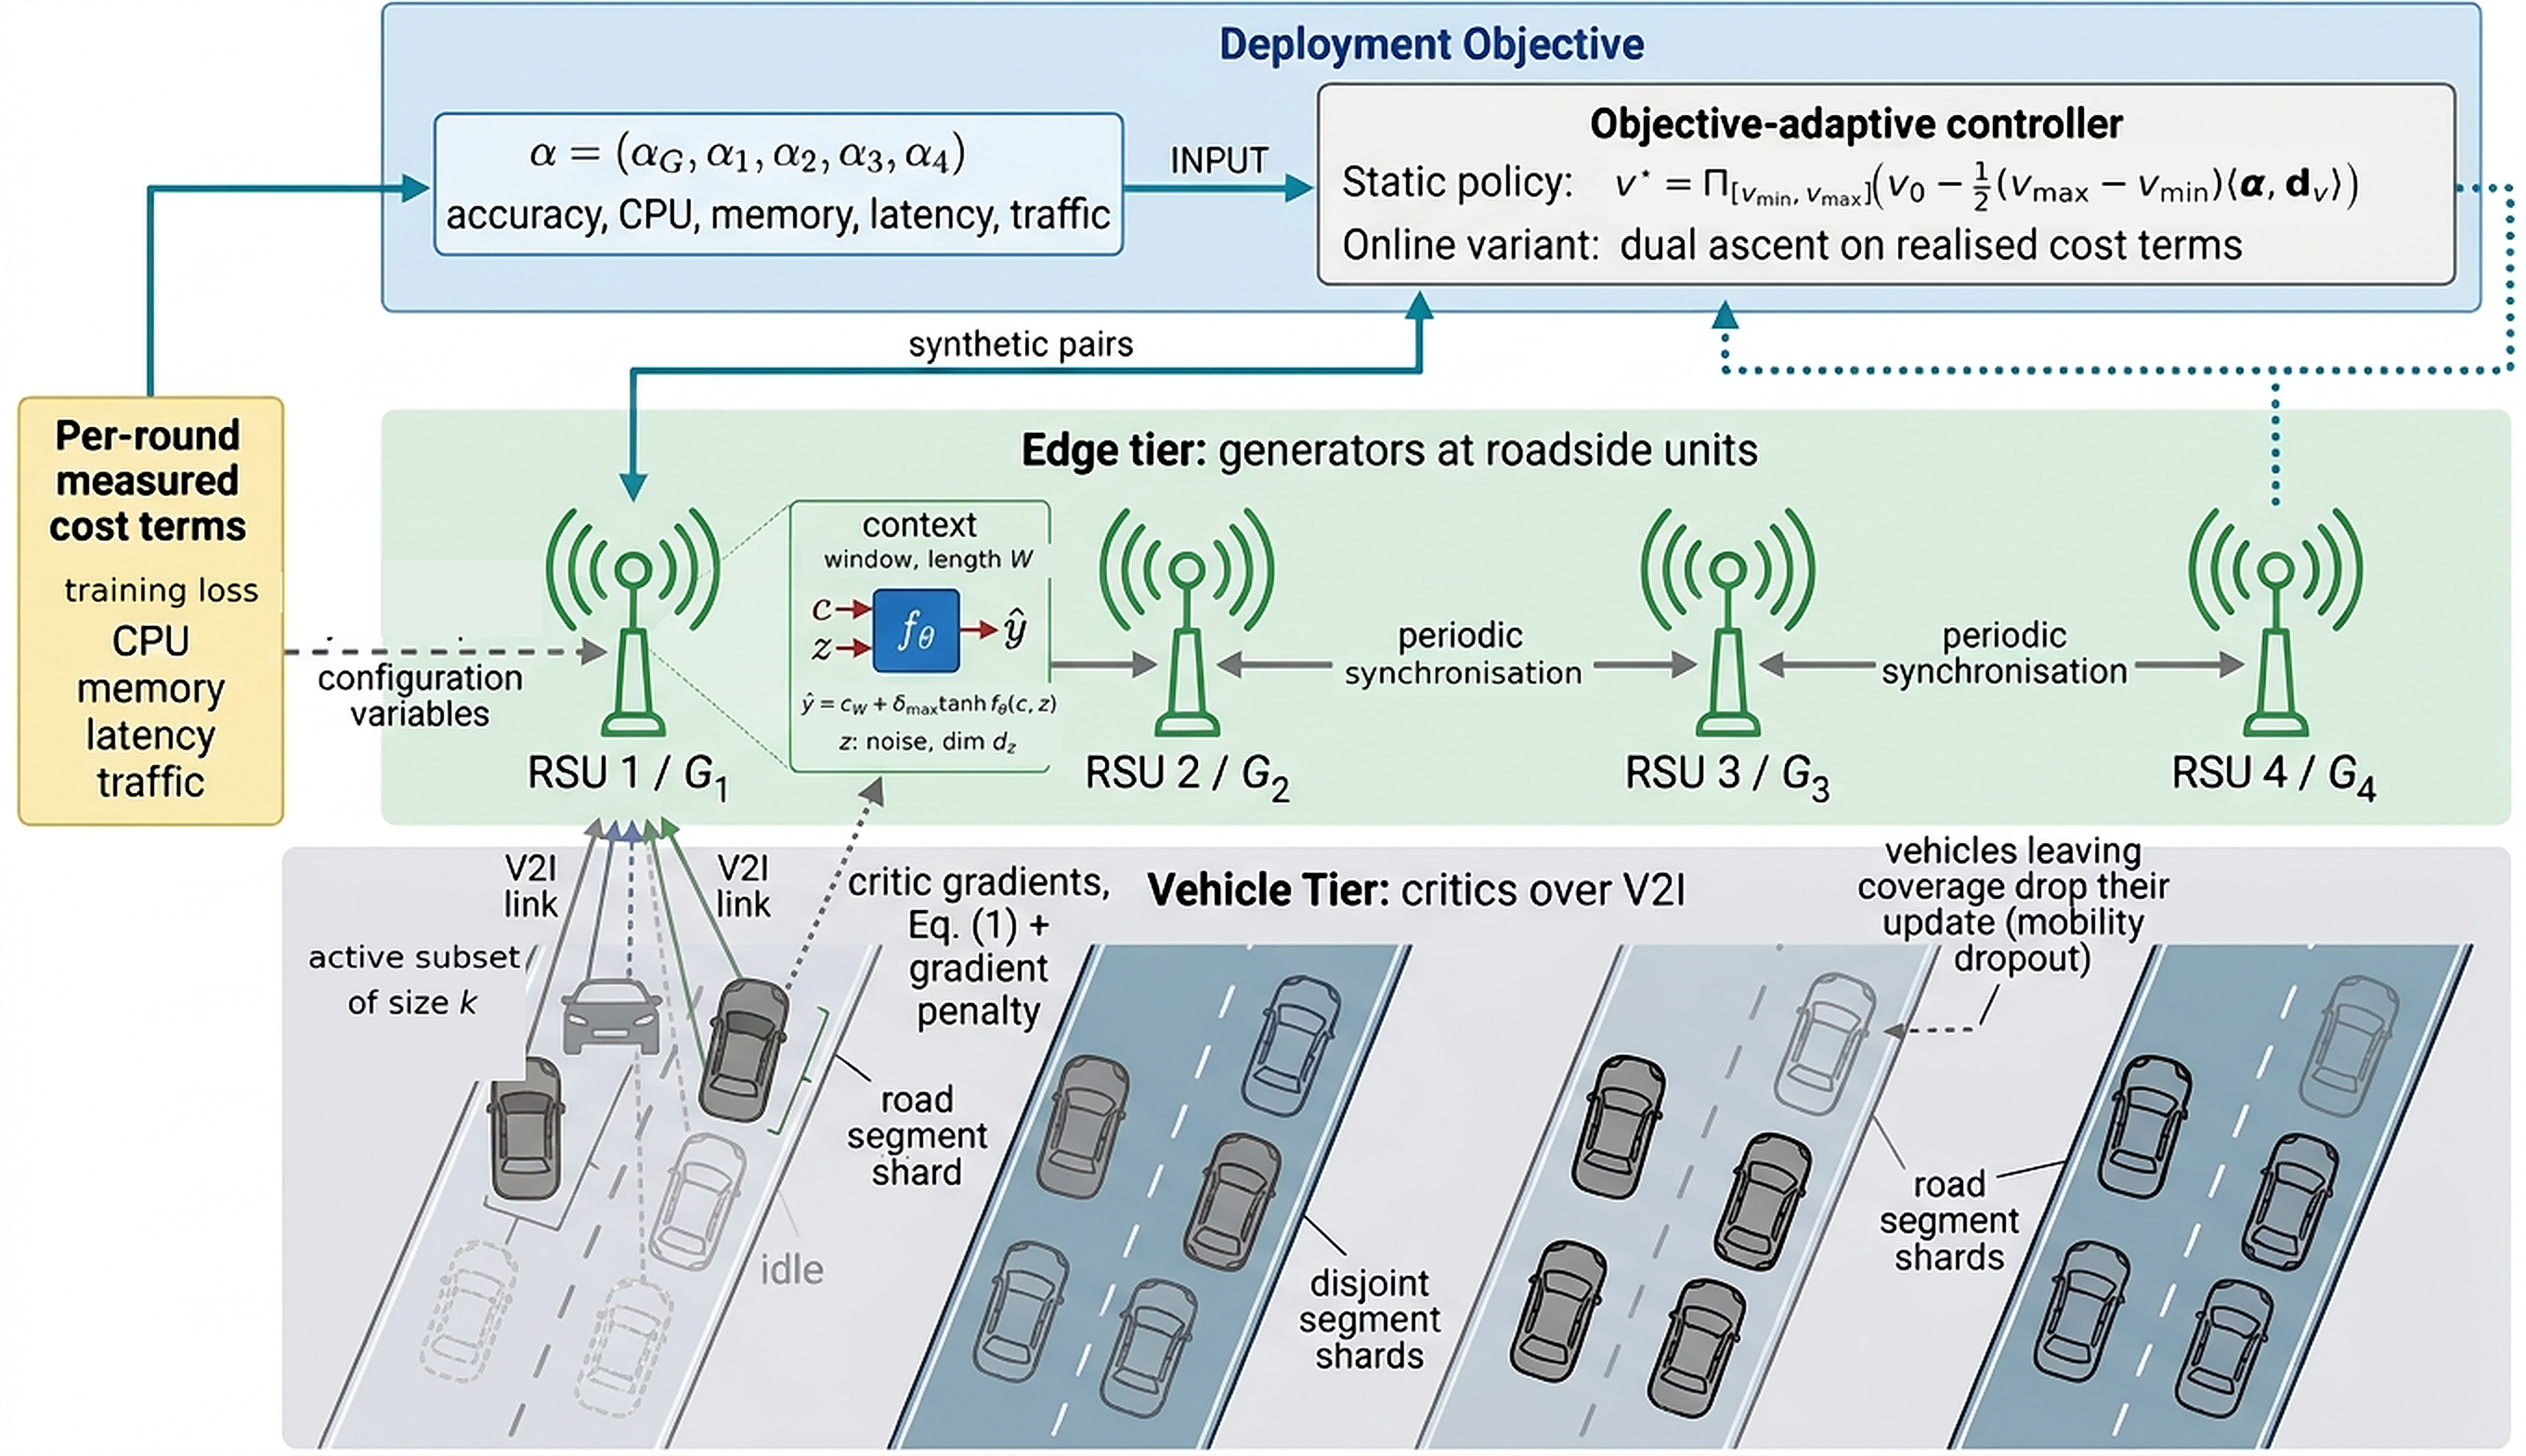
\includegraphics[width=0.92\textwidth]{fig_method_fixed_2x.png}
\caption{Architecture of the objective-adaptive MD-WGAN framework. The
deployment objective weights $\valpha$ are an input to the controller, which
sets the configuration $(k,E_G,S,\lambda_{\rm sup})$ of the edge tier. RSUs
host conditional generators; vehicles in each RSU's pool act as critics over
V2I links, with an active subset of size $k$ per round and the remainder idle.
Vehicles leaving coverage before the round closes drop their update. The dashed
path carries the realised cost terms back to the controller (online variant).}
\label{fig:arch}
\end{figure*}

\begin{table}[!t]
\centering
\caption{List of Symbols and Variables}
\label{tab:symbols}
\footnotesize
\begin{tabular}{ll}
\toprule
Symbol & Description \\
\midrule
$\mathcal{G}=\{1,\ldots,N_G\}$ & Set of generator nodes (RSUs) \\
$\mathcal{D}=\{1,\ldots,K\}$ & Set of discriminators (vehicles) \\
$\mathcal{D}_{g_i}$, $\mathcal{S}^{(t)}_{g_i}$ & Local pool of $g_i$; active subset at round $t$ \\
$k$, $K_S$ & Active subset size; active discriminators per RSU \\
$c$, $y$, $W$ & Context window of $W$ past feature vectors; next vector \\
$z\sim p_z$, $d_z$ & Latent input and its dimension \\
$G(c,z)$, $\hat{y}$ & Conditional generator output \\
$D_j(c,y)$ & Conditional critic score of pair $(c,y)$ \\
$\delta_{\max}$ & Bound of the generator's residual head \\
$\lambda_{\rm GP}$, $\lambda_{\rm sup}$, $k_s$ & Gradient-penalty, supervision weight; draws in best-of-$k_s$ \\
$h_{i,j}$, $d_{i,j}$, $\beta$ & Channel gain, distance, path-loss exponent \\
$R_{i,j}$, $B_n$, $P_{tx}$, $N_0$ & Rate, bandwidth, transmit power, noise PSD \\
$L^{(t)}_{\mathcal{D}_{g_i}}$, $T^{(t)}_{\mathcal{D}_{g_i}}$ & Round latency and network traffic of $g_i$ \\
$C^{(t)}_{\mathcal{D}_{g_i}}$, $M^{(t)}_{\mathcal{D}_{g_i}}$ & Compute (gradient-step units) and memory \\
$\valpha=(\alpha_G,\alpha_1,\ldots,\alpha_4)$ & Deployment objective weights, $\sum\alpha=1$ \\
$\J(\valpha;\mathbf{v})$ & Unified objective cost \\
$\mathbf{v}=(k,E_G,S,\lambda_{\rm sup})$ & Training configuration \\
$\vd_v\in\mathbb{R}^5$ & Cost direction of configuration variable $v$ \\
$\Pi_{[v_{\min},v_{\max}]}$ & Projection onto the admissible range \\
$\boldsymbol{\mu}$, $\eta$, $\rho$ & Dual multipliers, dual step, smoothing factor \\
$E_D$, $E_G$, $\mathcal{E}_D$, $\mathcal{E}_G$ & Epoch allocations and strategy sets \\
$U_D$, $U_G$, $\kappa$, $c^{\rm ep}$, $\gamma$ & Utilities, effectiveness rates, per-epoch cost, interference \\
$s_t$, $a_t$, $Q(s,a)$, $r_t$ & RL state, action, action value, reward \\
$S$, $S_{\rm sync}$ & Synchronisation interval; synchronisation steps per round \\
$\tau_j$, $T_r$ & Residence time of vehicle $j$; round interval \\
$d$, $B$ & Model parameters; batch size \\
\bottomrule
\end{tabular}
\end{table}

\subsection{Network and System Model}
\subsubsection{IoV Network Architecture}
We consider an IoV network consisting of:
\begin{itemize}
\item \textbf{Roadside Units (RSUs)}: $\mathcal{G}=\{1,\ldots,N_G\}$ RSUs host
      the generators and their local controllers, leveraging stationary,
      resource-rich infrastructure for adaptive decision making.
\item \textbf{Vehicles}: $\mathcal{D}=\{1,\ldots,K\}$ vehicles moving along the
      road act as discriminators, evaluating generated data against their own
      real samples under mobility constraints. Each generator $g_i$ is
      associated with a local pool $\mathcal{D}_{g_i}\subseteq\mathcal{D}$, of
      which a subset $\mathcal{S}^{(t)}_{g_i}$ of size $k$ is active in round $t$.
\item \textbf{V2I Communication}: RSUs and vehicles communicate over V2I
      wireless links.
\end{itemize}
As vehicles traverse the road, a discriminator may leave the coverage area of
one RSU and enter that of another, in which case its link is re-established
with the new generator. A vehicle whose residence time $\tau_j$ in the serving
cell expires before the round closes cannot return its critic feedback; its
update is lost and the generator proceeds with whatever arrived. We model this
\emph{mobility dropout} explicitly, with the probability of completing a round
of duration $T_r$ taken as $\exp(-T_r/\tau_j)$ under the standard memoryless
residence assumption, and every method in Section~\ref{sec:results} is
evaluated under it.

\subsubsection{Conditional WGAN Training Model}
Each training sample is a pair $(c,y)$, where the context $c$ is a window of
$W$ consecutive past feature vectors of one vehicle and $y$ is the subsequent
vector. The generator realises $\hat{y}=G(c,z)$ with $z\sim p_z$, and the
critic scores \emph{pairs}, so that the Wasserstein distance is taken between
conditional distributions. Following~\cite{arjovsky2017wgan}, discriminator
$D_j$ is trained with
\begin{equation}
\mathcal{L}_{D_j}=\mathbb{E}_{(c,y)\sim p_{\rm data}}\!\big[D_j(c,y)\big]
 -\mathbb{E}_{c,z}\!\big[D_j(c,G(c,z))\big]
 +\lambda_{\rm GP}\,\mathrm{GP}(D_j),
\label{eq:critic}
\end{equation}
where $\mathrm{GP}(D_j)=\mathbb{E}_{\hat{x}}\big[(\|\nabla_{\hat{x}}D_j(c,\hat{x})\|_2-1)^2\big]$
is the gradient penalty enforcing 1-Lipschitz continuity in $y$ along
interpolates $\hat{x}$ between real and generated samples.

The generator head predicts a \emph{bounded residual} about the last observed
frame $c_W$,
\begin{equation}
G(c,z)=c_W+\delta_{\max}\tanh\!\big(f_\theta(c,z)\big),
\label{eq:gen}
\end{equation}
where $f_\theta$ is a multilayer perceptron over an encoding of $c$
concatenated with $z$. The bound is both statistical and physical: an unbounded
head extrapolates without limit on contexts outside its training support, and a
vehicle's state cannot change arbitrarily between consecutive samples. Without
it we measured held-out errors two orders of magnitude beyond the data range.

\textbf{Ensemble feedback.} Each generator $g_i$ is updated against a weighted
ensemble of the critics that returned feedback in the round,
\begin{equation}
\mathcal{L}^{\rm adv}_{g_i}=-\sum_{j\in\mathcal{S}^{(t)}_{g_i}} w_j\,
 \mathbb{E}_{c,z}\!\big[D_j(c,G(c,z))\big],\qquad \sum_j w_j=1,
\label{eq:ensemble}
\end{equation}
with uniform weights by default (a performance-weighted variant is ablated in
Section~\ref{sec:ablation}).

\textbf{Supervision and predictive diversity.} A purely adversarial objective
does not constrain per-sample error: the critic rewards distributional realism,
which is compatible with arbitrarily large pointwise deviation. A supervised
term is therefore added. Applied naively, however, it creates the opposite
failure. Penalising every latent draw against the single observed future makes
the optimal response place all draws at the conditional mean, so the generator
stops using $z$. We measured exactly this: the spread of generator outputs
across latent draws fell to $\approx3\%$ of the data spread, and the nominal
$90\%$ predictive interval covered $26\%$ of targets. We therefore use
winner-take-all (best-of-$k_s$) supervision in the manner of the variety loss
of~\cite{gupta2018socialgan}, penalising only the closest of $k_s$ draws,
\begin{equation}
\mathcal{L}_{\rm sup}=\mathbb{E}_{(c,y)}\Big[\min_{m=1,\ldots,k_s}
 \ell\big(G(c,z^{(m)}),\,y\big)\Big],
\label{eq:sup}
\end{equation}
with $\ell$ the smooth-$\ell_1$ loss, which leaves the remaining draws free to
cover alternative futures. The generator objective is
\begin{equation}
\mathcal{L}_{g_i}=\mathcal{L}^{\rm adv}_{g_i}+\lambda_{\rm sup}\,\mathcal{L}_{\rm sup}.
\label{eq:gloss}
\end{equation}
Section~\ref{sec:calibration} quantifies the effect: PICP rises from $0.22$ to
$0.73$ at unchanged RMSE. A mode-seeking regulariser~\cite{mao2019msgan} is
evaluated as an alternative.

\subsection{Communication Model}
\subsubsection{Wireless Channel}
The link between generator $g_i$ and discriminator $D_j$ experiences channel
gain $h_{i,j}$ following the log-distance path-loss model~\cite{rappaport2002wireless},
\begin{equation}
h_{i,j}=h_0\Big(\frac{d_0}{d_{i,j}}\Big)^{\beta},
\label{eq:pathloss}
\end{equation}
where $d_{i,j}$ is the distance, $\beta$ the path-loss exponent and $h_0$ the
reference gain at $d_0$. Vehicles move between rounds, so $d_{i,j}$ and hence
the channel each discriminator sees change as it traverses the coverage zone.

\subsubsection{Data Transmission}
The achievable rate follows the Shannon--Hartley capacity~\cite{rappaport2002wireless},
\begin{equation}
R_{i,j}=B_n\log_2\!\Big(1+\frac{P_{tx}h_{i,j}}{N_0B_n}\Big),
\label{eq:rate}
\end{equation}
with bandwidth $B_n$, transmit power $P_{tx}$ and noise spectral density $N_0$.
A synchronisation step exchanges a payload of $b$ bytes on the downlink
(synthetic samples) and the uplink (critic feedback) with every active
discriminator, and the generator waits for all of them, so the round latency is
governed by the slowest link:
\begin{align}
L^{(t)}_{\mathcal{D}_{g_i}}&=S^{(t)}_{\rm sync}\max_{j\in\mathcal{S}^{(t)}_{g_i}}
 \Big(\frac{2\cdot 8b}{R_{i,j}}+2t_{\rm proc}\Big)+t^{(t)}_{\rm comp},
\label{eq:latency}\\
T^{(t)}_{\mathcal{D}_{g_i}}&=S^{(t)}_{\rm sync}\,\eta_{\rm proto}\sum_{j\in\mathcal{S}^{(t)}_{g_i}}2b,
\label{eq:traffic}
\end{align}
where $S^{(t)}_{\rm sync}=\lceil E_G/S\rceil$ is the number of synchronisation
steps actually taken in the round (one per $S$ generator updates), $t_{\rm proc}$
a per-message processing delay, $\eta_{\rm proto}$ the protocol overhead
factor and $t^{(t)}_{\rm comp}$ the compute time of the round. This latency is
the round-trip of a federated synchronisation cycle, not the inference-time
latency of the trained generator. Both the synchronisation interval $S$ and the
subset size $k$ enter~(\ref{eq:latency})--(\ref{eq:traffic}) directly, which is
what makes them useful control variables.

\subsection{Computation Model}
Each generator allocates computing resources to its associated discriminators,
and each vehicular node has CPU and memory limits. Wall-clock CPU percentage on
a shared host measures the scheduler and thread count rather than the method,
so we quantify compute as the \emph{algorithmic work} performed in the round,
in units of batch-gradient steps: critic steps are weighted by the batch they
process and generator steps by the number of critics they query,
\begin{align}
C^{(t)}_{\mathcal{D}_{g_i}}&=\frac{B}{10^3}\Big(E_D\,|\mathcal{S}^{(t)}_{g_i}|
 +E_G\,|\mathcal{S}^{(t)}_{g_i}|\Big),
\label{eq:cpu}\\
M^{(t)}_{\mathcal{D}_{g_i}}&=\frac{1}{|\mathcal{S}^{(t)}_{g_i}|}\sum_{j\in\mathcal{S}^{(t)}_{g_i}}
 \mathrm{MEM}^{\rm used}_j(t),
\label{eq:mem}
\end{align}
with measured resident memory $\mathrm{MEM}^{\rm used}_j$. Measured process CPU
is retained in the released records for reference.

% =====================================================================
\section{Problem Formulation}
\label{sec:problem}

\subsection{Unified Objective}
For each generator $g_i$ and round $t$, the deployment scores training by a
weighted cost over training quality and four resource terms,
\begin{equation}
\begin{split}
\J(\valpha;\mathbf{v})=\;&\alpha_G\,\tilde{\mathcal{L}}^{(t)}_{g_i}
 +\alpha_1\frac{C^{(t)}_{\mathcal{D}_{g_i}}}{C_{\max}}
 +\alpha_2\frac{M^{(t)}_{\mathcal{D}_{g_i}}}{M_{\max}}\\
 &+\alpha_3\frac{L^{(t)}_{\mathcal{D}_{g_i}}}{L_{\max}}
 +\alpha_4\frac{T^{(t)}_{\mathcal{D}_{g_i}}}{T_{\max}},
\end{split}
\label{eq:obj}
\end{equation}
subject to
\begin{align}
C^{(t)}_{\mathcal{D}_{g_i}}\le C_{\max},\quad
M^{(t)}_{\mathcal{D}_{g_i}}\le M_{\max},&\qquad\forall g_i\in\mathcal{G},
\label{eq:c1}\\
L^{(t)}_{\mathcal{D}_{g_i}}\le L_{\max},\quad
T^{(t)}_{\mathcal{D}_{g_i}}\le T_{\max},&\qquad\forall g_i\in\mathcal{G},
\label{eq:c2}\\
\big|\mathrm{Loss}^{t+1}_v-\mathrm{Loss}^{t}_v\big|\le\epsilon,&\qquad\forall v\in\mathcal{G}\cup\mathcal{D},
\label{eq:c3}
\end{align}
where $\tilde{\mathcal{L}}$ is the normalised training term (the Wasserstein
estimate during training; CRPS for post-hoc scoring), $C_{\max}$ is the work of
the most expensive schedule the configuration can select, $M_{\max}$ the
maximum memory capacity, $L_{\max}$ the maximum acceptable latency and
$T_{\max}$ the traffic of synchronising with the whole pool every epoch. Because
$\sum_i\alpha_i=1$, the coefficients define a convex combination over five
competing objectives, so increasing any one necessarily reduces the relative
influence of the others. The problem is to choose the model parameters
$\theta_G,\{\theta_{D_j}\}$, the active subsets $\mathcal{S}^{(t)}_{g_i}$, the
epoch allocation $(E_D,E_G)$ and -- the focus of this paper -- the training
configuration $\mathbf{v}$ so as to minimise~(\ref{eq:obj}).

\subsection{Objective Function Components}
\begin{itemize}
\item \textbf{Training quality} ($\alpha_G\tilde{\mathcal{L}}$): the Wasserstein
      estimate of~(\ref{eq:critic}), sigmoid-squashed so that it is
      commensurable with the normalised resource terms; when configurations are
      compared after training, the terminal CRPS is used, being strictly proper.
\item \textbf{Computation} ($\alpha_1C/C_{\max}$): normalised algorithmic work
      of~(\ref{eq:cpu}), penalising processor demand on the vehicles.
\item \textbf{Memory} ($\alpha_2M/M_{\max}$): normalised resident memory
      of~(\ref{eq:mem}), keeping memory available for other tasks.
\item \textbf{Communication latency} ($\alpha_3L/L_{\max}$): normalised round
      latency of~(\ref{eq:latency}).
\item \textbf{Network traffic} ($\alpha_4T/T_{\max}$): normalised transmission
      volume of~(\ref{eq:traffic}), penalising congestion of the shared channel.
\end{itemize}

\subsection{Configuration Variables and the Fixed-Configuration Gap}
\label{sec:gap}
Four variables of the training process drive distinct terms of~(\ref{eq:obj})
in opposite directions, and are therefore the natural control variables:
\begin{itemize}
\item the \textbf{active subset size} $k=|\mathcal{S}^{(t)}_{g_i}|$: more critics
      lower the training term but raise all four cost terms through
      (\ref{eq:latency})--(\ref{eq:cpu});
\item the \textbf{generator epoch budget} $E_G$: more generator updates per
      round converge faster but cost compute and, through
      $S_{\rm sync}$, latency and traffic;
\item the \textbf{synchronisation interval} $S$: synchronising less often cuts
      traffic and latency at the price of staler critic feedback;
\item the \textbf{supervision weight} $\lambda_{\rm sup}$: stronger supervision
      lowers point error but, as Section~\ref{sec:calibration} shows, degrades
      distributional quality and calibration.
\end{itemize}
We write $\mathbf{v}=(k,E_G,S,\lambda_{\rm sup})\in\mathcal{V}$ for the
configuration and $\J(\valpha;\mathbf{v})$ for the resulting cost. Every
federated GAN framework we are aware of chooses one $\mathbf{v}^\circ$ before
training and reports $\J(\valpha;\mathbf{v}^\circ)$ for one or more $\valpha$.
Since each variable moves at least two terms of~(\ref{eq:obj}) in opposite
directions, the minimiser $\mathbf{v}^\star(\valpha)=\arg\min_{\mathbf{v}}\J(\valpha;\mathbf{v})$
depends on $\valpha$ unless the cost directions of all variables are parallel,
and a fixed $\mathbf{v}^\circ$ incurs the gap
$\J(\valpha;\mathbf{v}^\circ)-\J(\valpha;\mathbf{v}^\star(\valpha))\ge0$ for every
$\valpha\neq\valpha^\circ$. Section~\ref{sec:scen} measures this gap: it is
$35$--$75\%$ of the cost of the strongest fixed baseline, and $58$--$85\%$ of
our own fixed configuration's cost. The objective-adaptive problem is therefore
\begin{equation}
\min_{\mathbf{v}\in\mathcal{V}}\ \J(\valpha;\mathbf{v})
\quad\text{given }\valpha\text{ at deployment time},
\label{eq:adaptprob}
\end{equation}
solved jointly with the per-round selection and allocation decisions.

% =====================================================================
\section{Objective-Adaptive Multi-Discriminator Framework}
\label{sec:framework}

The framework coordinates generator and discriminator training through five
interacting mechanisms (Fig.~\ref{fig:workflow}): a configuration step that
reads $\valpha$ (Step~0), an adaptive decision engine selecting which
discriminators participate (Step~1), a game-theoretic step allocating training
epochs (Step~2), distributed training and synchronisation (Step~3), and
monitoring that closes the loop (Step~4). Algorithm~\ref{alg:cycle} gives the
cycle; the steps are detailed in turn.

\begin{figure}[!t]
\centering
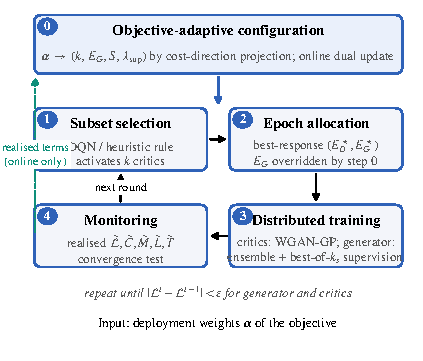
\includegraphics[width=\columnwidth]{fig2_workflow.pdf}
\caption{Adaptation cycle of the proposed framework. Step~0 maps the deployment
weights $\valpha$ to a training configuration; Steps~1--4 repeat each round.
The dashed feedback path is used by the online variant only.}
\label{fig:workflow}
\end{figure}

\begin{algorithm}[!t]
\caption{Objective-adaptive adaptation cycle for one generator $g_i$ and its pool $\mathcal{D}_{g_i}$}
\label{alg:cycle}
\begin{algorithmic}[1]
\REQUIRE deployment weights $\valpha$; directions $\{\vd_v\}$; bounds
$[v_{\min},v_{\max}]$; initial $\theta_G,\{\theta_{D_j}\}$; thresholds $\epsilon_G,\epsilon_D$
\ENSURE trained generator and critics
\STATE $t\leftarrow0$; $\boldsymbol{\mu}\leftarrow\mathbf{1}$; initialise replay buffer $\mathcal{B}$
\STATE \textbf{Step 0 (static):} $\mathbf{v}\leftarrow$ Eq.~(\ref{eq:policy}) with $\valpha$
\REPEAT
  \STATE \textbf{Step 0 (online):} if enabled, $\mathbf{v}\leftarrow$ Eqs.~(\ref{eq:share})--(\ref{eq:onlinepolicy}) with $\valpha\odot\boldsymbol{\mu}$
  \STATE \textbf{Step 1:} $\mathcal{S}^{(t)}_{g_i}\leftarrow$ top-$k$ of $\pi(s_t)$ \hfill$\triangleright$ DQN or heuristic rule
  \STATE \textbf{Step 2:} $(E^\star_D,E^\star_G)\leftarrow\textsc{BestResponse}(U_D,U_G)$; $E_G\leftarrow E_G$ from $\mathbf{v}$
  \STATE \textbf{Step 3:} for $j\in\mathcal{S}^{(t)}_{g_i}$: $E_D$ critic steps on~(\ref{eq:critic});
         drop vehicles whose residence expired;
         $E_G$ generator steps on~(\ref{eq:gloss}), synchronising every $S$ steps
  \STATE \textbf{Step 4:} measure $(\tilde{\mathcal{L}},\tilde{C},\tilde{M},\tilde{L},\tilde{T})$;
         update $\boldsymbol{\mu}$ by~(\ref{eq:mult}); update $\hat\kappa,\hat c^{\rm ep}$ by~(\ref{eq:kappahat});
         $s_{t+1}\leftarrow f(\cdot)$; store transition in $\mathcal{B}$; DQN replay step
  \STATE $t\leftarrow t+1$
\UNTIL{$|\mathcal{L}^t_G-\mathcal{L}^{t-1}_G|<\epsilon_G$ and $|\mathcal{L}^t_D-\mathcal{L}^{t-1}_D|<\epsilon_D$}
\end{algorithmic}
\end{algorithm}

\subsection{Step 0: Objective-Adaptive Configuration}
\label{sec:controller}
\subsubsection{Cost Directions}
Each configuration variable $v\in\{k,E_G,S,\lambda_{\rm sup}\}$ carries a
direction $\vd_v\in\mathbb{R}^5$ whose entries give the sign and relative
magnitude of the effect of \emph{raising} $v$ on the five terms
of~(\ref{eq:obj}), ordered (training, compute, memory, latency, traffic).
The entries (Table~\ref{tab:ctrl}) are set from the controlled sweeps of
Section~\ref{sec:sensitivity} rather than assumed: raising $k$ from $1$ to $5$
lowers the training term and raises compute, latency and traffic monotonically
(Table~\ref{tab:scale}); raising $E_G$ lowers the training term and raises
compute and, through $S_{\rm sync}$, latency and traffic; raising $S$ lowers
latency and traffic and mildly compute at the price of the training term; and
raising $\lambda_{\rm sup}$ affects the training term only. The cost of raising
$v$ under a deployment with weights $\valpha$ is then the inner product
\begin{equation}
\chi_v(\valpha)=\langle\valpha,\vd_v\rangle,
\label{eq:direction}
\end{equation}
positive when the terms $v$ makes more expensive outweigh those it improves.

\subsubsection{Static Policy}
The static policy maps $\valpha$ to a configuration once, before training, by
moving each variable against its cost from a reference configuration $v_0$:
\begin{equation}
v^{\star}=\Pi_{[v_{\min},v_{\max}]}\Big(v_0-\tfrac12\,(v_{\max}-v_{\min})\,
 \langle\valpha,\vd_v\rangle\Big),
\label{eq:policy}
\end{equation}
with $\Pi$ the projection onto the admissible range and integer variables
rounded. The step is bounded at half the range so that no single weighting
drives a variable to a corner. The supervision mode is set to plain
conditional-mean supervision when $\alpha_G>0.35$ -- a strongly
accuracy-weighted deployment does not need the calibration that
best-of-$k_s$ buys, and plain supervision gives marginally better point error --
and to best-of-$k_s$ otherwise. Selecting a configuration costs one inner
product of length five per variable and nothing at runtime.

\subsubsection{Online Controller}
The online variant retains~(\ref{eq:policy}) as its base and adds a dual update
on the terms each round actually realises, so that the configuration tracks the
objective rather than a prediction of it. Let
$\mathbf{u}^{(t)}\in[0,1]^5$ be the normalised terms realised in round $t$ and
$\bar{\mathbf{u}}^{(t)}=\rho\bar{\mathbf{u}}^{(t-1)}+(1-\rho)\mathbf{u}^{(t)}$
their exponential moving average. Each term's share of the realised total is
compared with the share its weight entitles it to,
\begin{equation}
\xi^{(t)}_i=\frac{\bar{u}^{(t)}_i}{\sum_l\bar{u}^{(t)}_l}-\alpha_i,
\label{eq:share}
\end{equation}
and a term consuming more than its share raises its multiplier,
\begin{equation}
\mu^{(t+1)}_i=\Pi_{[\mu_{\min},\mu_{\max}]}\big(\mu^{(t)}_i\exp(\eta\,\xi^{(t)}_i)\big),
\label{eq:mult}
\end{equation}
which is the standard multiplicative dual update for a weighted-sum
objective~\cite{boyd2004convex}. The effective weights
$\tilde{\valpha}=\valpha\odot\boldsymbol{\mu}/\|\valpha\odot\boldsymbol{\mu}\|_1$
replace $\valpha$ in~(\ref{eq:policy}),
\begin{equation}
v^{(t+1)}=\Pi_{[v_{\min},v_{\max}]}\Big(v_0-\tfrac12\,(v_{\max}-v_{\min})\,
 \langle\tilde{\valpha}^{(t)},\vd_v\rangle\Big),
\label{eq:onlinepolicy}
\end{equation}
so a term over-consuming its budget pushes the variables that drive it
downward and a term under budget relaxes them. This can respond to conditions
the static map cannot anticipate -- congestion, unexpectedly slow nodes, an
early plateau -- at the cost of a few vector operations per round.
Section~\ref{sec:scen} reports that the static policy is the better choice in
four of the five weightings evaluated, so the online variant is presented as an
explored alternative rather than the recommended configuration. Both
controllers are deliberately small: the selection experiments of
Section~\ref{sec:selection} show that elaborate search buys nothing in this
setting, so the controller is a handful of bounded updates rather than another
learned policy.

\begin{table}[!t]
\centering
\caption{Controller parameters: admissible ranges, measured cost directions
$\vd_v$ over (training, compute, memory, latency, traffic), and dual-update
constants.}
\label{tab:ctrl}
\footnotesize
\begin{tabular}{lccc}
\toprule
Variable & Range $[v_{\min},v_{\max}]$ & Reference $v_0$ & Direction $\vd_v$ \\
\midrule
$k$ & $[1,5]$ & 3 & $(-1,\,+1,\,+1,\,+1,\,+1)$ \\
$E_G$ & $[2,25]$ & 5 & $(-1,\,+1,\,0,\,+1,\,+1)$ \\
$S$ & $[1,4]$ & 1 & $(+1,\,-0.3,\,0,\,-1,\,-1)$ \\
$\lambda_{\rm sup}$ & $[0,25]$ & 10 & $(-0.5,\,0,\,0,\,0,\,0)$ \\
\midrule
\multicolumn{4}{l}{Online: $\eta=0.25$, $\rho=0.7$, $[\mu_{\min},\mu_{\max}]=[0.25,4]$} \\
\bottomrule
\end{tabular}
\end{table}

\subsection{Step 1: Adaptive Decision Engine}
\label{sec:step1}
Each generator maintains a selector that activates $k$ discriminators from its
local pool. The learned selector is an independent Deep Q-Network (DQN) agent
per generator.

\subsubsection{RL Formulation}
\begin{itemize}
\item \textbf{State space}: $\mathcal{S}\in\mathbb{R}^7$, aggregating for $g_i$
      and its pool the average critic loss, average critic score,
      communication latency, compute, memory, network traffic, and the
      previous round's critic score:
      \begin{equation}
      s_t=[\bar{\mathcal{L}}_D,\ \bar{s}_D,\ \mathrm{lat},\ \mathrm{cpu},\
           \mathrm{mem},\ \mathrm{traf},\ \bar{s}^{(t-1)}_D].
      \label{eq:state}
      \end{equation}
\item \textbf{Action space}: one Q-value per candidate in the local pool,
      $|\mathcal{A}|=K_{\rm local}$; the top-$k$ by Q-value form
      $\mathcal{S}^{(t)}_{g_i}$. Per-candidate scoring avoids the
      $\binom{K_{\rm local}}{k}$ blow-up of enumerating subsets, at the cost
      of not modelling interactions between simultaneously selected critics.
\item \textbf{Network}: fully connected $[128,128,|\mathcal{A}|]$ with ReLU
      activations, target network and experience replay (Table~\ref{tab:dqn}).
\end{itemize}
The action value is updated by
\begin{equation}
Q(s_t,a_t)\leftarrow Q(s_t,a_t)+\alpha_{\rm lr}\Big[r^{(t)}_{g_i}
 +\gamma\max_{a}Q(s_{t+1},a)-Q(s_t,a_t)\Big],
\label{eq:q}
\end{equation}
with $\epsilon$-greedy exploration decaying as
$\epsilon_t=\max(\epsilon_{\min},\epsilon_0\epsilon^t_{\rm decay})$.

\subsubsection{Reward}
To align the agent with~(\ref{eq:obj}), the per-round reward balances training
progress against normalised resource cost,
\begin{equation}
r^{(t)}_{g_i}=w_1\frac{\Delta\mathcal{L}^{(t)}_{g_i}}{\mathcal{L}^{(t-1)}_{g_i}}
 -w_2\hat{L}^{(t)}-w_3\hat{T}^{(t)}-w_4\hat{C}^{(t)}-w_5\hat{M}^{(t)},
\label{eq:reward}
\end{equation}
where $\Delta\mathcal{L}^{(t)}_{g_i}=\mathcal{L}^{(t-1)}_{g_i}-\mathcal{L}^{(t)}_{g_i}$
is the improvement in the Wasserstein estimate between consecutive rounds,
hats denote terms normalised to $[0,1]$, and $\sum_iw_i=1$.

\subsubsection{Non-learning Rules}
Because the state of~(\ref{eq:state}) is dominated by quantities a direct rule
can also read, we evaluate the DQN against seven alternatives with everything
else held fixed: uniform random-$k$; round-robin; greedy-by-loss (the $k$
critics with the highest smoothed loss, i.e.\ those currently hardest to fool);
lazy-greedy and genetic search over a submodular set objective combining shard
similarity, link latency and completion probability; a residence-aware rule
that weights informativeness by the survival probability $\exp(-T_r/\tau_j)$
and link rate; and activating the whole pool. Section~\ref{sec:selection}
reports the comparison.

\begin{table}[!t]
\centering
\caption{DQN Hyperparameters}
\label{tab:dqn}
\footnotesize
\begin{tabular}{ll}
\toprule
Parameter & Value \\
\midrule
State dimension $|\mathcal{S}|$ & 7 \\
Network & FC $[128,128,|\mathcal{A}|]$, ReLU \\
Discount $\gamma$ & 0.99 \\
Exploration $\epsilon_0$ / $\epsilon_{\min}$ / $\epsilon_{\rm decay}$ & 1.0 / 0.01 / 0.995 \\
Replay buffer / minibatch & 10\,000 / 64 \\
Target-network sync & every 10 updates \\
Optimiser / loss & Adam ($10^{-3}$) / MSE \\
Reward weights $(w_1,\ldots,w_5)$ & $(0.2,0.2,0.2,0.2,0.2)$ \\
\bottomrule
\end{tabular}
\end{table}

\subsection{Step 2: Game-Theoretic Epoch Allocation}
\label{sec:step2}
The interaction between critics and generator over the round's training budget
is modelled as a two-player game over discrete strategy sets $\mathcal{E}_D$
and $\mathcal{E}_G$ of epoch allocations. For a strategy pair $(E_D,E_G)$ the
utilities trade training effectiveness against resource cost and against an
interference term reflecting degradation caused by the opponent:
\begin{align}
U_D(E_D,E_G)&=f_D(E_D)-\lambda_D\,c^{\rm ep}_D\,E_D-\gamma\,f_G(E_G),
\label{eq:utilD}\\
U_G(E_D,E_G)&=f_G(E_G)-\lambda_G\,c^{\rm ep}_G\,E_G-\gamma\,f_D(E_D),
\label{eq:utilG}
\end{align}
with diminishing-returns effectiveness
$f_D(E)=1-e^{-\kappa_DE}$, $f_G(E)=1-e^{-\kappa_GE}$,
per-epoch costs $c^{\rm ep}_D,c^{\rm ep}_G$ scaled by $\lambda_D,\lambda_G$,
and interference coefficient $\gamma$.

\subsubsection{Online Re-estimation}
The parameters $\kappa$ and $c^{\rm ep}$ are not constants. At the end of each
round they are re-estimated from what the round achieved: given a realised
relative loss improvement $r$ over $E$ epochs, inverting the effectiveness
model gives
\begin{equation}
\hat{\kappa}=-\frac{\ln(1-r)}{E},\qquad
\hat{c}^{\rm ep}=t_{\rm epoch},
\label{eq:kappahat}
\end{equation}
with $t_{\rm epoch}$ the measured wall-clock seconds per epoch, both smoothed
by an exponential moving average and clamped to keep the model well posed. This matters for a reason worth stating plainly: with fixed
parameters the allocation is identical in every round and the mechanism reduces
to a constant schedule. The ablation of Section~\ref{sec:ablation} includes that
static variant so the contribution of online adaptation can be separated.

\subsubsection{Best-Response Search}
Given $\mathcal{E}_D$ and $\mathcal{E}_G$, the coordinator computes an
approximate equilibrium by a two-pass best-response search: for each
$E_D\in\mathcal{E}_D$ the generator's best response maximising $U_G$ is found,
yielding a candidate pair; symmetrically for each $E_G\in\mathcal{E}_G$; the
pair with the higher joint payoff $U_D+U_G$ is selected. Because this evaluates
best responses in a bounded number of passes rather than iterating to a fixed
point, we refer to it as best-response coordination rather than a converged
Nash equilibrium. Its cost is $\mathcal{O}(|\mathcal{E}_D||\mathcal{E}_G|)$,
constant in network size.

\subsubsection{Interaction with Step 0}
The generator budget $E_G$ is one of the four controlled variables, and the
controller's value overrides the coordinator's $E^\star_G$: $E_G$ is the
variable that trades convergence speed against compute, latency and traffic,
so it is the one the objective weighting most needs to move. The coordinator
retains control of $E_D$. Without the controller (the fixed-configuration
baseline of Section~\ref{sec:results}), the coordinator sets both; we observed
that with converged estimates it drives $E_G$ to the top of its strategy set
within five rounds, which is precisely the behaviour a weighted objective that
values traffic or compute must be able to override.

\begin{table}[!t]
\centering
\caption{Game-Theoretic Coordination Parameters}
\label{tab:game}
\footnotesize
\begin{tabular}{ll}
\toprule
Parameter & Value \\
\midrule
Initial effectiveness rates $\kappa_D$ / $\kappa_G$ & 0.05 / 0.10 \\
Initial per-epoch cost $c^{\rm ep}_D$ / $c^{\rm ep}_G$ (s) & 0.3 / 0.8 \\
Cost weights $\lambda_D$ / $\lambda_G$ & 0.05 / 0.05 \\
Interference coefficient $\gamma$ & 0.7 \\
Strategy sets $\mathcal{E}_D$ / $\mathcal{E}_G$ & $\{45,50,\ldots,75\}$ / $\{2,3,\ldots,15\}$ \\
EMA factor for online estimates & 0.6 \\
Fixed schedule (ablation) $(E_D,E_G)$ & $(50,5)$ \\
\bottomrule
\end{tabular}
\end{table}

\subsection{Step 3: Distributed Training and Synchronisation}
\label{sec:step3}
With the active subset from Step~1 and the allocation from Step~2, each active
discriminator $D_j$ performs $E_D$ gradient steps on~(\ref{eq:critic}) over its
own partition, with gradient clipping. Vehicles whose residence time expires
during the round are dropped from the ensemble. The generator then performs
$E_G$ gradient steps on~(\ref{eq:gloss}) against the ensemble of critics that
returned feedback, exchanging parameters with the active discriminators every
$S$ generator steps; the number of exchanges $S_{\rm sync}=\lceil E_G/S\rceil$
is what the latency and traffic terms of~(\ref{eq:latency})--(\ref{eq:traffic})
count. Discriminators are trained independently and in parallel, each on a
distinct local partition.

\subsection{Step 4: Monitoring and Convergence}
\label{sec:step4}
The monitoring step collects, per round and per generator: the realised
Wasserstein estimate; algorithmic work and resident memory; round latency and
traffic from the channel model; the number of dropped vehicles; and held-out
accuracy metrics. These feed (i) the online controller
(\ref{eq:share})--(\ref{eq:onlinepolicy}), (ii) the coordinator's re-estimation
(\ref{eq:kappahat}), (iii) the RL state~(\ref{eq:state}) and
reward~(\ref{eq:reward}), and (iv) the multi-level convergence criterion
\begin{equation}
C_{\rm loss}=\big(|\mathcal{L}^{(t)}_G-\mathcal{L}^{(t-1)}_G|<\epsilon_G\big)
 \wedge\big(|\mathcal{L}^{(t)}_D-\mathcal{L}^{(t-1)}_D|<\epsilon_D\big),
\label{eq:conv}
\end{equation}
which requires both sides to stabilise before training terminates.

\subsection{Complexity Analysis}
\label{sec:complexity}
Let $N_G$ be the number of RSUs, $K$ the number of vehicles, $K_{\rm local}$
the local pool size, $K_S\le K_{\rm local}$ the active subset, $d$ the parameter
count of a model, $B$ the batch size and $E$ the epochs per round.
\begin{itemize}
\item \textbf{Configuration (Step 0)}: the static policy costs four inner
      products of length five, once; the online controller adds
      $\mathcal{O}(5)$ operations per round. Both are $\mathcal{O}(1)$ in every
      scale variable.
\item \textbf{Selection (Step 1)}: one DQN forward pass,
      $\mathcal{O}(|\mathcal{S}|\cdot128+128^2+128\,K_{\rm local})$. Because
      $K_{\rm local}$ is bounded by design -- scaling the system adds RSUs
      rather than growing a pool -- this is $\mathcal{O}(1)$ in $N_G$ and $K$.
\item \textbf{Allocation (Step 2)}: $\mathcal{O}(|\mathcal{E}_D||\mathcal{E}_G|)$,
      constant.
\item \textbf{Training (Step 3)}: $\mathcal{O}(E\,d\,B)$ per round, with critic
      steps parallel across vehicles; adding nodes does not increase it.
\item \textbf{Communication}: $\mathcal{O}(S_{\rm sync}N_GK_Sd)$ per round --
      linear in RSUs and active critics, and proportional to the number of
      synchronisation steps.
\end{itemize}
The controller acts on exactly the factors of the communication term that are
under the framework's control: $K_S$ through $k$, and $S_{\rm sync}$ through
$E_G$ and $S$. Table~\ref{tab:complexity} summarises; Section~\ref{sec:comm}
measures the communication term over IEEE 802.11p.

\begin{table}[!t]
\centering
\caption{Summary of Scalability Analysis}
\label{tab:complexity}
\footnotesize
\begin{tabular}{lll}
\toprule
Aspect & Complexity & Implication \\
\midrule
Configuration & $\mathcal{O}(1)$ & Independent of scale \\
Selection & $\mathcal{O}(K_{\rm local})$ & Bounded pool; constant in $N_G,K$ \\
Allocation & $\mathcal{O}(|\mathcal{E}_D||\mathcal{E}_G|)$ & Constant \\
Computation & $\mathcal{O}(E\,d\,B)$ & Parallel across nodes \\
Communication & $\mathcal{O}(S_{\rm sync}N_GK_Sd)$ & Linear in $N_G$, $K_S$; controller sets $K_S$, $S_{\rm sync}$ \\
\bottomrule
\end{tabular}
\end{table}

% =====================================================================
\section{Experimental Setup}
\label{sec:setup}

\subsection{Simulation Environment}
The framework is implemented in PyTorch as a seed-controlled harness in which
every mechanism of Section~\ref{sec:framework} is an independently switchable
configuration field, so that each ablation arm is traceable to one named
configuration and seed. The vehicular channel of~(\ref{eq:pathloss})--(\ref{eq:traffic})
drives per-round latency and traffic during training; the synchronisation round
is additionally simulated at the packet level with the ns-3 IEEE 802.11p stack
(Section~\ref{sec:comm}). Table~\ref{tab:sim} lists the parameters. Experiments
ran on an Amazon EC2 m5.4xlarge instance (16 vCPUs, 64\,GB). All results are
means over five independent seeds unless stated otherwise; runs are exactly
reproducible per seed.

\begin{table}[!t]
\centering
\caption{Simulation Parameters}
\label{tab:sim}
\footnotesize
\begin{tabular}{ll}
\toprule
Parameter & Value \\
\midrule
\multicolumn{2}{l}{\emph{Data and training}} \\
Dataset / features & NGSIM; speed, accel., lane, headway, lateral pos. \\
Context window $W$ / latent dim.\ $d_z$ & 8 / 16 \\
Partitioning & by road segment; one global scaler \\
Tracks per node / test fraction & $\le400$ / 0.2 (whole-track split) \\
RSUs $N_G$ / pool per RSU / active $k$ & 2 (2--6) / 5 (3--8) / 3 (1--5) \\
Rounds / batch $B$ / learning rates & 60 / 64 / $10^{-4}$ (Adam, $G$ and $D$) \\
$\lambda_{\rm GP}$ / $\lambda_{\rm sup}$ / $k_s$ / $\delta_{\max}$ & 10 / 10 / 8 / 1$\sigma$ \\
Hidden width / encoder width & 128 / 64 \\
Mobility dropout & enabled for all methods \\
\multicolumn{2}{l}{\emph{Channel model (training-time cost terms)}} \\
Bandwidth $B_n$ / $P_{tx}$ / $N_0$ & 10\,MHz / 23\,dBm / $-174$\,dBm/Hz \\
Path-loss exponent $\beta$ / cell radius & 2.7 / 400\,m \\
Vehicle speed / round interval $T_r$ & 15--60\,m/s / 1\,s \\
Protocol overhead / processing delay & 8\% / 2\,ms per message \\
\multicolumn{2}{l}{\emph{ns-3 packet-level simulation}} \\
Standard / PHY rate / channel & IEEE 802.11p / OFDM 6\,Mb/s, 10\,MHz / 5.9\,GHz \\
Propagation & log-distance, ref.\ loss 47.86\,dB at 1\,m \\
Mobility / area & random waypoint, 15--60\,m/s / 600\,m $\times$ 600\,m \\
Vehicles / RSUs / $k$ / payload & 8--40 / 2--8 / 1--5 / 512--4096\,B \\
Rounds / seeds & 40 / 5 \\
\bottomrule
\end{tabular}
\end{table}

\subsection{Dataset}
Training and evaluation use the NGSIM trajectory dataset~\cite{ngsim}. Each
sample is a five-dimensional feature vector -- longitudinal speed and
acceleration, lane identifier, headway distance to the lead vehicle and lateral
position -- computed per vehicle per time step, organised into (context,
target) pairs with $W=8$. Splits are taken over \emph{whole vehicle tracks}, so
no test context overlaps a training one, and scalers are fitted on training
data only. Trajectories are partitioned across discriminators \emph{by road
segment}, so each holds a locally coherent and genuinely distinct shard, and
all nodes share one global feature scaler. This choice is consequential: with
per-node scaling every shard becomes approximately standard normal, the
measured spread of per-node feature means across nodes falls to zero, and no
selection or adaptation mechanism can be distinguished from any other.
Section~\ref{sec:partition} evaluates the alternatives.

\subsection{Evaluation Metrics}
Accuracy is measured on the held-out set between each predicted next-step
vector $\hat{y}_i=G(c_i,z)$ and its ground-truth continuation $y_i$:
\begin{itemize}
\item \textbf{RMSE} and \textbf{MAE}, retained for comparability, computed
      against the mean over 16 latent draws (the Bayes-optimal point estimate);
\item \textbf{CRPS}~\cite{gneiting2007crps}, over 20 draws per context: the
      primary accuracy metric, because it is strictly proper and cannot be
      improved by collapsing to the conditional mean;
\item \textbf{minADE$_{20}$}~\cite{gupta2018socialgan}: error of the closest of
      20 draws, crediting coverage of the plausible set of futures;
\item \textbf{PICP}: fraction of targets inside the model's own nominal $90\%$
      interval, ideal $0.90$; and \textbf{mode coverage}, the fraction of
      per-feature histogram bins of the real data reached by generated samples;
\item \textbf{Rounds and compute to target}: training rounds and cumulative work
      units~(\ref{eq:cpu}) to first reach RMSE $\le0.86$, reported with the
      fraction of seeds that reach it (seeds that never do are not averaged
      away);
\item \textbf{Latency} (s) and \textbf{traffic} (bytes) per round
      from~(\ref{eq:latency})--(\ref{eq:traffic}); \textbf{compute} in work
      units; \textbf{memory} in MB;
\item \textbf{Objective cost} $\J(\valpha;\mathbf{v})$ of~(\ref{eq:obj}) with
      terminal CRPS as the training term and the remaining terms averaged over
      the final $20\%$ of rounds, min--max normalised across the configurations
      compared so that the five terms are commensurable.
\end{itemize}
Every reported difference is accompanied by a paired Wilcoxon signed-rank test
across common seeds, Holm-corrected within each family of comparisons. Paired
tests are used because the seed effect is large relative to the architectural
effects: the seed-to-seed spread of the full framework is $0.073$ RMSE, which
exceeds most between-method differences reported in this literature. With
$n=5$ seeds the smallest attainable $p$ is $0.062$, so the absence of
$p<0.05$ at $n=5$ is weak evidence of no effect rather than evidence of none.

\subsection{Baseline Comparisons}
\label{sec:baselines}
All baselines share the conditional backbone of~(\ref{eq:critic})--(\ref{eq:gen}),
the data partitioning, optimiser settings, mobility dropout and seeds; only the
coordination strategy differs, so differences are attributable to coordination
rather than to architecture, data handling or tuning.
\begin{itemize}
\item \textbf{HVS-GAN}~\cite{wu2024hvsgan}: each scheduled vehicle trains a
      complete local GAN; a server aggregates generators by FedAvg weighted by
      sample count; a DDPG agent (Ornstein--Uhlenbeck exploration, target
      networks, soft updates) schedules the top-$k$ vehicles from per-vehicle
      (loss, capability, cost, staleness), with capability drawn in $[0.4,1.0]$
      scaling local epochs and participation cost in $[0.5,1.5]$ entering the
      reward.
\item \textbf{FedAvg-GAN}: identical to HVS-GAN with uniform random
      participation, isolating exactly what the DDPG scheduler contributes.
\item \textbf{MD-GAN}~\cite{hardy2019mdgan}: one central generator, every
      discriminator active each round, discriminators swapped between workers
      every five rounds.
\item \textbf{Proposed (fixed)}: the framework of Section~\ref{sec:framework}
      at a fixed configuration $(k,E_G,S,\lambda_{\rm sup})=(3,\cdot,1,10)$ with
      $E_G$ set by the coordinator, greedy-by-loss selection and
      best-of-$k_s$ supervision; and \textbf{Proposed (fixed, DQN)}, the same
      with DQN selection and conditional-mean supervision, i.e.\ the
      configuration of our earlier design.
\item \textbf{Proposed (adaptive)}: the framework with Step~0 enabled, reporting
      for each weighting whichever of the static and online variants attains
      the lower cost; both are shown in Section~\ref{sec:scen}.
\end{itemize}
These are our re-implementations; absolute values may differ from the original
publications because dataset, backbone and protocol are held common by design.
Our earlier early-update MD-GAN~\cite{kaleibar2025mascots} was evaluated under a
different pipeline and is not included, since its numbers would not be
comparable under this protocol.

\subsection{Reproducibility}
The implementation, the ns-3 simulation, every experiment configuration and the
complete per-seed run records are available at
\url{https://github.com/farhoudjk/MD-WGAN}.

% =====================================================================
\section{Results}
\label{sec:results}

\subsection{Accuracy and Convergence Against Baselines}
\label{sec:sota}
Table~\ref{tab:metrics} and Fig.~\ref{fig:conv} compare the fixed-configuration
framework with the three baselines. The proposed configuration attains the best
point error (RMSE $0.776$ versus $0.836$ for MD-GAN and $0.897$ for HVS-GAN, a
gap of two to four seed standard deviations), the best multi-modal error
(minADE $1.075$) and markedly the best calibration (PICP $0.721$ against
$0.40$--$0.47$). Fig.~\ref{fig:cost} gives the operationally important result:
the framework first reaches RMSE $\le0.86$ after $6.4$ rounds and $187$ work
units, against $36$ rounds and $1267$ units for MD-GAN -- $5.6\times$ fewer
rounds at $6.8\times$ less computation -- and MD-GAN reaches it in only four of
five seeds, while HVS-GAN and FedAvg-GAN do not reach it within 60 rounds in
any seed.

\textbf{Two results do not favour the proposed configuration.} MD-GAN attains
a better terminal CRPS ($0.371$ versus $0.396$), and Fig.~\ref{fig:conv}(b)
shows it overtaking the proposed configuration near round~45: our advantage is
the cost of reaching a given accuracy, not the distributional score at
convergence. Our fixed configuration also transmits the most per round
($17.2$\,MB against $9.6$\,MB for MD-GAN) and has the highest latency. These are
genuine losses, and they are exactly the terms the adaptive controller of
Section~\ref{sec:scen} is designed to move.

Finally, HVS-GAN and FedAvg-GAN agree to within $0.001$ on every metric: in
this setting the DDPG scheduler of~\cite{wu2024hvsgan} does not outperform
uniform random participant selection. Section~\ref{sec:selection} reports the
corresponding result for our own learned selector.

\begin{table*}[!t]
\centering
\caption{Predictive quality on held-out NGSIM continuations and per-round cost
under a common protocol. Mean\,$\pm$\,s.d.\ over five seeds. PICP is best at
its nominal $0.90$; all other metrics are better when lower. No fixed
configuration dominates.}
\label{tab:metrics}
\begin{tabular}{lcccccccc}
\toprule
Method & RMSE $\downarrow$ & CRPS $\downarrow$ & minADE $\downarrow$ & PICP $\rightarrow0.90$ & Coverage $\uparrow$ & Compute/round $\downarrow$ & Latency (s) $\downarrow$ & Traffic (MB) $\downarrow$ \\
\midrule
MD-GAN~\cite{hardy2019mdgan} & 0.836\,$\pm$\,0.032 & \textbf{0.371\,$\pm$\,0.008} & 1.131\,$\pm$\,0.024 & 0.470\,$\pm$\,0.024 & 0.941 & 17.6 & 1.56 & \textbf{9.57} \\
HVS-GAN~\cite{wu2024hvsgan} & 0.897\,$\pm$\,0.035 & 0.400\,$\pm$\,0.010 & 1.302\,$\pm$\,0.040 & 0.403\,$\pm$\,0.046 & \textbf{0.991} & 7.5 & 1.08 & 12.17 \\
FedAvg-GAN & 0.897\,$\pm$\,0.035 & 0.400\,$\pm$\,0.011 & 1.303\,$\pm$\,0.041 & 0.404\,$\pm$\,0.026 & \textbf{0.991} & \textbf{7.0} & \textbf{1.02} & 11.37 \\
Proposed (fixed, DQN) & \textbf{0.775\,$\pm$\,0.030} & 0.408\,$\pm$\,0.021 & 1.194\,$\pm$\,0.059 & 0.222\,$\pm$\,0.028 & 0.912 & 16.6 & 1.93 & 17.09 \\
Proposed (fixed) & 0.776\,$\pm$\,0.029 & 0.396\,$\pm$\,0.017 & \textbf{1.075\,$\pm$\,0.042} & \textbf{0.721\,$\pm$\,0.011} & 0.923 & 16.6 & 2.16 & 17.23 \\
\bottomrule
\end{tabular}
\end{table*}

\begin{figure*}[!t]
\centering
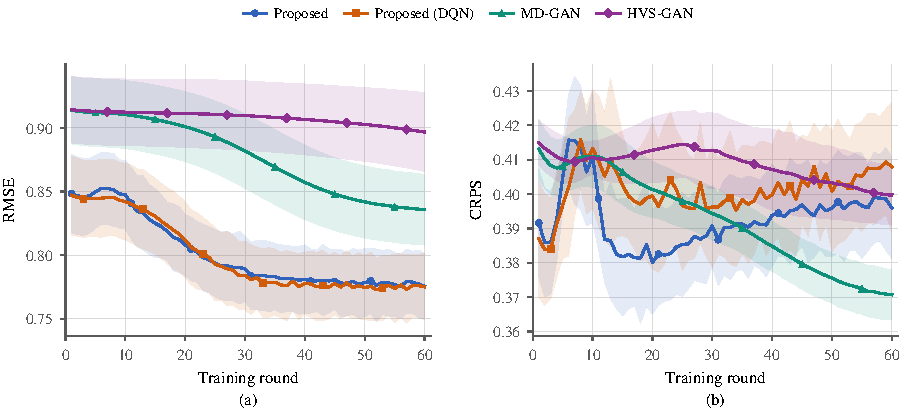
\includegraphics[width=\textwidth]{fig1_convergence.pdf}
\caption{Convergence against federated GAN baselines: (a) RMSE and (b) CRPS
versus training round, with 95\% confidence bands over five seeds. MD-GAN
overtakes the proposed configuration on CRPS near round~45.}
\label{fig:conv}
\end{figure*}

\begin{figure*}[!t]
\centering
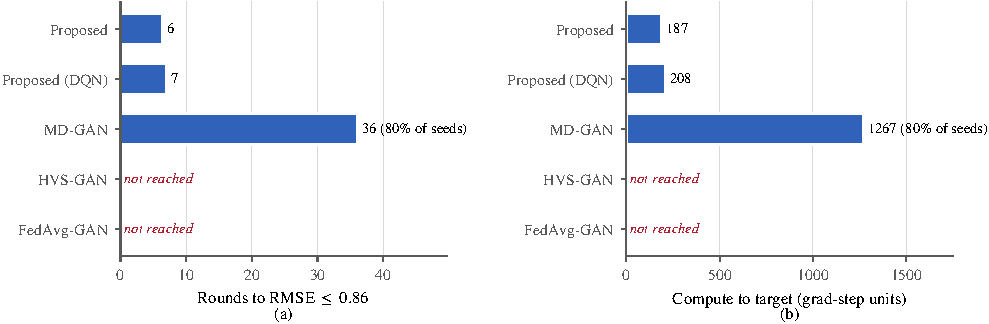
\includegraphics[width=\textwidth]{fig2_cost_to_target.pdf}
\caption{Cost of first reaching RMSE $\le0.86$: (a) training rounds and
(b) gradient-step work. Annotations give the fraction of seeds reaching the
target; HVS-GAN and FedAvg-GAN do not reach it in any seed within 60 rounds.}
\label{fig:cost}
\end{figure*}

\subsection{Objective Cost Under Five Deployment Weightings}
\label{sec:scen}
Following the application scenarios of our earlier formulation, we evaluate
five weightings of~(\ref{eq:obj}): \emph{balanced}
$(0.2,0.2,0.2,0.2,0.2)$; \emph{accuracy-oriented}, $\alpha_G=0.4$ and $0.15$
elsewhere, for high-fidelity data synthesis; \emph{delay-sensitive},
$\alpha_3=0.4$, for safety-critical tasks; \emph{network-overhead-oriented},
$\alpha_4=0.4$, for bandwidth-limited environments; and
\emph{resource-constrained}, $\alpha_1=\alpha_2=0.29$, for low-power nodes.
Table~\ref{tab:scenario} and Fig.~\ref{fig:scenario} score every configuration
under each weighting, each column with its own $\valpha$.

Three observations follow. First, the ordering and the gaps among the fixed
configurations change with the weighting: MD-GAN's deficit to the best fixed
baseline is $0.17$ under the balanced weighting and $0.035$ under the
accuracy weighting, and our two fixed configurations exchange places between
the accuracy and delay columns. Second, \textbf{our own fixed configurations
are the weakest rows of the table} under every weighting ($0.60$--$0.74$
against $0.34$--$0.46$ for FedAvg-GAN): the point accuracy and calibration they
attain in Table~\ref{tab:metrics} are bought with the highest compute and
traffic, and a weighted cost charges for them. Third, the adaptive framework is
best in all five columns, improving on the strongest fixed baseline by $35\%$
(accuracy) to $75\%$ (network), with the direction consistent across all five
seeds in every column. The gain is attributable to adaptation, not to the
multi-discriminator architecture, and we state this rather than attributing it
to the framework as a whole.

Fig.~\ref{fig:breakdown} decomposes the cost into its weighted terms. Under the
balanced weighting the fixed configurations are dominated by compute and
traffic; the adaptive configuration removes most of both while its training
term is the smallest of any row. Table~\ref{tab:terms} gives the realised
quantities behind the normalised scores: the adaptive configurations hold CRPS
at $0.376$--$0.377$ -- better than our fixed configuration ($0.396$) and within
$0.006$ of MD-GAN ($0.371$) -- at $9.8$--$12.9$ work units per round against
$16.6$--$17.6$, and at $0.8$--$4.2$\,MB of traffic against $9.6$--$17.2$\,MB,
an order of magnitude less. The price is point error: RMSE rises from $0.776$
to $0.836$--$0.840$, the level of MD-GAN, and PICP falls from $0.72$ to
$0.63$--$0.65$. A deployment that weights point error above all is served by
the accuracy-weighted column, where the controller keeps more critics and more
generator epochs (Table~\ref{tab:config}).

\begin{table*}[!t]
\centering
\caption{Normalised objective cost $\J(\valpha)$ of~(\ref{eq:obj}) under five
deployment weightings; each column is evaluated with its own $\valpha$. Lower
is better. Five seeds per cell; terms are min--max normalised across all
configurations so the five components are commensurable.}
\label{tab:scenario}
\begin{tabular}{lccccc}
\toprule
Method & Balanced & Accuracy & Delay & Network & Resource \\
\midrule
MD-GAN~\cite{hardy2019mdgan}   & 0.562 & 0.451 & 0.551 & 0.555 & 0.639 \\
HVS-GAN~\cite{wu2024hvsgan}    & 0.424 & 0.436 & 0.369 & 0.491 & 0.408 \\
FedAvg-GAN                     & 0.395 & 0.416 & 0.338 & 0.457 & 0.379 \\
Proposed (fixed, DQN)          & 0.650 & 0.631 & 0.678 & 0.735 & 0.593 \\
Proposed (fixed)               & 0.658 & 0.601 & 0.722 & 0.743 & 0.602 \\
\midrule
\textbf{Proposed (adaptive)}   & \textbf{0.171} & \textbf{0.269} & \textbf{0.184} & \textbf{0.112} & \textbf{0.159} \\
\quad selected variant         & static & online & static & static & static \\
\quad gain vs.\ best fixed     & 56.6\% & 35.2\% & 45.4\% & 75.4\% & 58.1\% \\
\quad paired Wilcoxon $p$      & 0.062 & 0.062 & 0.062 & 0.062 & 0.062 \\
\bottomrule
\end{tabular}
\end{table*}

\begin{figure*}[!t]
\centering
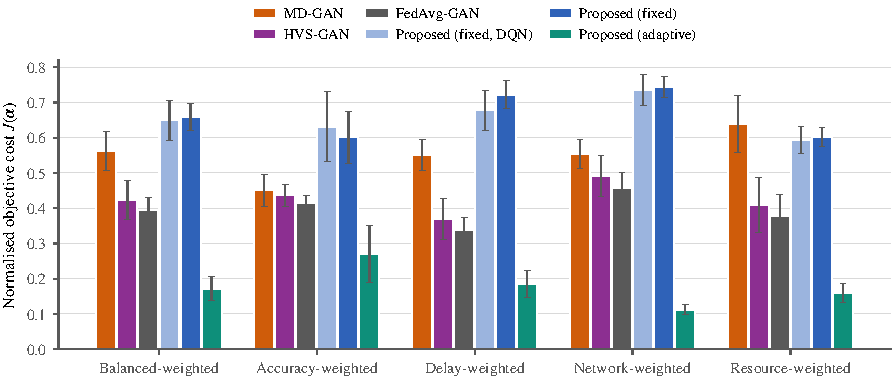
\includegraphics[width=\textwidth]{fig8_scenario_cost.pdf}
\caption{Normalised objective cost of every configuration under each
deployment weighting (lower is better; error bars are 95\% confidence
intervals over five seeds). The adaptive framework is lowest in every group;
the ordering of the fixed configurations changes between groups.}
\label{fig:scenario}
\end{figure*}

\begin{figure*}[!t]
\centering
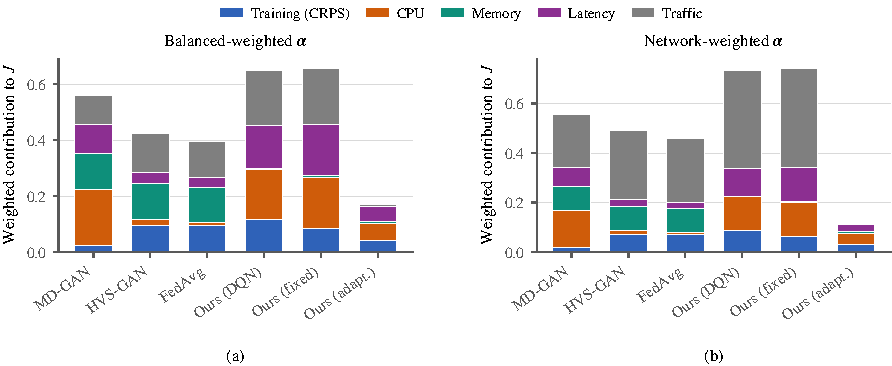
\includegraphics[width=\textwidth]{fig12_cost_breakdown.pdf}
\caption{Decomposition of the objective cost into its $\valpha$-weighted terms
under (a) the balanced and (b) the network-oriented weighting. The fixed
configurations are dominated by compute and traffic; the adaptive configuration
removes most of both while attaining the smallest training term.}
\label{fig:breakdown}
\end{figure*}

\begin{table*}[!t]
\centering
\caption{Realised terms behind Table~\ref{tab:scenario}, before normalisation.
CRPS, RMSE and PICP are terminal values; compute (work units per round),
resident memory, round latency and traffic are means over the final 20\% of
rounds. Five seeds throughout.}
\label{tab:terms}
\begin{tabular}{lccccccc}
\toprule
Configuration & CRPS & RMSE & PICP & Compute & Mem.\ (MB) & Lat.\ (s) & Traffic (MB) \\
\midrule
MD-GAN & 0.371\,$\pm$\,0.008 & 0.836 & 0.47 & 17.6 & 470 & 1.56 & 9.57 \\
HVS-GAN & 0.400\,$\pm$\,0.010 & 0.897 & 0.40 & 7.5 & 470 & 1.08 & 12.17 \\
FedAvg-GAN & 0.400\,$\pm$\,0.011 & 0.897 & 0.40 & 7.0 & 468 & 1.02 & 11.37 \\
Proposed (fixed, DQN) & 0.408\,$\pm$\,0.021 & 0.775 & 0.22 & 16.6 & 389 & 1.93 & 17.09 \\
Proposed (fixed) & 0.396\,$\pm$\,0.017 & 0.776 & 0.72 & 16.6 & 392 & 2.16 & 17.23 \\
\midrule
Adaptive, balanced $\valpha$ (static) & 0.377\,$\pm$\,0.016 & 0.839 & 0.65 & 9.8 & 393 & 1.17 & 1.49 \\
Adaptive, accuracy $\valpha$ (online) & 0.376\,$\pm$\,0.018 & 0.836 & 0.63 & 12.9 & 393 & 1.48 & 4.19 \\
Adaptive, delay $\valpha$ (static) & 0.377\,$\pm$\,0.016 & 0.840 & 0.65 & 9.8 & 393 & 1.15 & 0.77 \\
Adaptive, network $\valpha$ (static) & 0.377\,$\pm$\,0.016 & 0.840 & 0.65 & 9.8 & 394 & 1.06 & 0.77 \\
Adaptive, resource $\valpha$ (static) & 0.377\,$\pm$\,0.016 & 0.839 & 0.65 & 9.8 & 393 & 1.02 & 1.49 \\
\bottomrule
\end{tabular}
\end{table*}

\subsection{Static Versus Online Adaptation}
\label{sec:modes}
Table~\ref{tab:modes} and Fig.~\ref{fig:modes} separate the two controllers
from the fixed configuration under each weighting. Merely \emph{knowing} the
objective -- the static map of~(\ref{eq:policy}), applied once -- lowers cost
by $50$--$85\%$ relative to the fixed configuration and is the better variant
in four of five weightings, where its gain is $73$--$85\%$. The online controller wins only under the
accuracy-oriented weighting, where its dual update relaxes the compute and
traffic terms as the training term's share grows, and is otherwise worse than
the static map by $0.07$--$0.21$. The feedback loop therefore does not earn its
complexity in this setting, and we recommend the static policy; the online
variant is reported because the question of whether feedback helps is the one a
reader would ask, and the answer here is that it mostly does not.

Table~\ref{tab:config} shows what the static policy actually selects. Under
every weighting but the accuracy-oriented one it reduces the active subset from
three critics to two and the generator budget from its reference value of five
epochs (the coordinator, left to itself, drives it to fifteen) to two, and
under the delay and network weightings it additionally halves the
synchronisation frequency; under the accuracy weighting it keeps three critics,
a larger generator budget and plain supervision. Fig.~\ref{fig:trace} traces a
network-weighted run: the fixed coordinator drives $E_G$ to the top of its
strategy set within five rounds and holds it there, so traffic accumulates
linearly to roughly $1$\,GB over 60 rounds; the static policy holds $E_G=2$ and
$k=2$ throughout, accumulating $45$\,MB; the online controller starts from the
same point and relaxes $k$ to three and $E_G$ to four after round~30 as the
training term's share rises, at a modest traffic cost. All three attain
comparable CRPS by round~60, with the adaptive variants better and far less
variable in the early rounds.

\begin{table}[!t]
\centering
\caption{Objective cost of the proposed framework with no controller, the static
policy and the online controller; each row is scored under its own weighting.
Mean over five seeds; $p$ is a paired Wilcoxon test of the better adaptive
variant against the fixed configuration ($0.062$ is the smallest value
attainable at $n=5$).}
\label{tab:modes}
\begin{tabular}{lcccrc}
\toprule
Weighting & Fixed & Static & Online & Gain & $p$ \\
\midrule
Balanced & 0.662 & \textbf{0.171} & 0.348 & 74.1\% & 0.062 \\
Accuracy & 0.641 & 0.319 & \textbf{0.269} & 58.0\% & 0.062 \\
Delay & 0.693 & \textbf{0.184} & 0.256 & 73.4\% & 0.062 \\
Network & 0.731 & \textbf{0.112} & 0.221 & 84.6\% & 0.062 \\
Resource & 0.601 & \textbf{0.159} & 0.368 & 73.6\% & 0.062 \\
\bottomrule
\end{tabular}
\end{table}

\begin{table}[!t]
\centering
\caption{Configuration selected by the static policy~(\ref{eq:policy}) under
each weighting from the reference $(k,E_G,S,\lambda_{\rm sup})=(3,5,1,10)$, and
the mean $(k,E_G)$ realised by the online controller over 60 rounds.}
\label{tab:config}
\begin{tabular}{lcccccc}
\toprule
Weighting & $k$ & $E_G$ & $S$ & $\lambda_{\rm sup}$ & Supervision & Online $\bar{k}/\bar{E}_G$ \\
\midrule
Balanced & 2 & 2 & 1 & 11.2 & best-of-$k_s$ & 2.4\,/\,2.9 \\
Accuracy & 3 & 4 & 1 & 12.5 & mean & 2.1\,/\,2.6 \\
Delay & 2 & 2 & 2 & 10.9 & best-of-$k_s$ & 2.0\,/\,2.9 \\
Network & 2 & 2 & 2 & 10.9 & best-of-$k_s$ & 2.0\,/\,3.0 \\
Resource & 2 & 2 & 1 & 10.9 & best-of-$k_s$ & 2.2\,/\,3.3 \\
\bottomrule
\end{tabular}
\end{table}

\begin{figure}[!t]
\centering
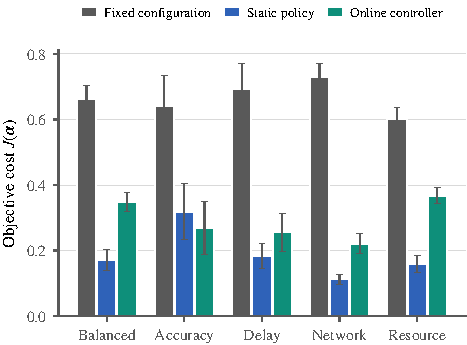
\includegraphics[width=\columnwidth]{fig9_adapt_modes.pdf}
\caption{Objective cost of the fixed configuration, the static policy and the
online controller under each weighting (95\% confidence intervals over five
seeds). The static policy is better in four of five weightings.}
\label{fig:modes}
\end{figure}

\begin{figure*}[!t]
\centering
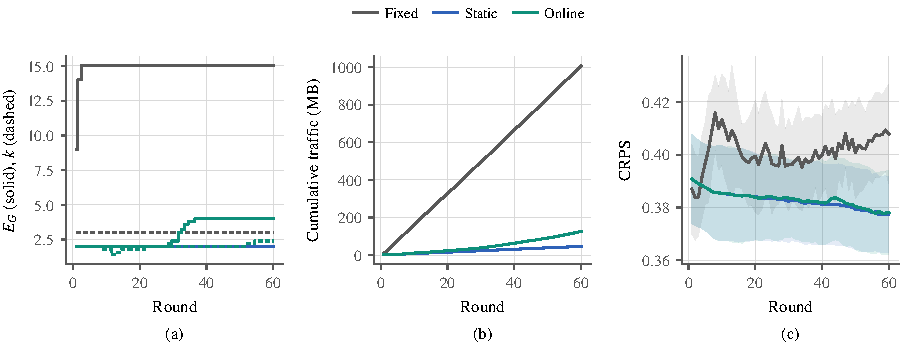
\includegraphics[width=\textwidth]{fig11_controller_trace.pdf}
\caption{Trace of a network-weighted run for the fixed configuration, the
static policy and the online controller (means over five seeds): (a) generator
budget $E_G$ (solid) and active subset $k$ (dashed) per round; (b) cumulative
traffic; (c) CRPS with 95\% confidence bands.}
\label{fig:trace}
\end{figure*}

\subsection{Controller Ablation: Which Variable Carries the Result}
\label{sec:knobs}
Table~\ref{tab:knobs} and Fig.~\ref{fig:knobs} enable one configuration
variable at a time under the network and resource weightings, leaving the
others at their reference values. The active subset size alone recovers most of
the available benefit: $0.198$ against $0.167$ for all four variables jointly
under the network weighting, from $0.771$ for the fixed configuration. The
generator budget is the second most effective variable, the synchronisation
interval third, and the supervision weight -- which affects only the training
term -- the least. Under the resource weighting, tuning $k$ alone ($0.263$)
\emph{outperforms} tuning all four jointly ($0.338$): the linear direction
model of~(\ref{eq:direction}) does not represent interaction between variables
and over-corrects when several move together. We report this rather than tune
it away; modelling the interaction is left to future work.

\begin{table}[!t]
\centering
\caption{Controller ablation: objective cost with a single variable enabled and
the remainder at their reference values (five seeds).}
\label{tab:knobs}
\begin{tabular}{lcc}
\toprule
Variable enabled & Network-weighted & Resource-weighted \\
\midrule
None (fixed configuration)              & 0.771 & 0.714 \\
Active subset size $k$                  & \textbf{0.198} & \textbf{0.263} \\
Generator epochs $E_G$                  & 0.310 & 0.503 \\
Synchronisation interval $S$            & 0.351 & 0.584 \\
Supervision weight $\lambda_{\rm sup}$  & 0.423 & 0.527 \\
All four jointly                        & 0.167 & 0.338 \\
\bottomrule
\end{tabular}
\end{table}

\begin{figure*}[!t]
\centering
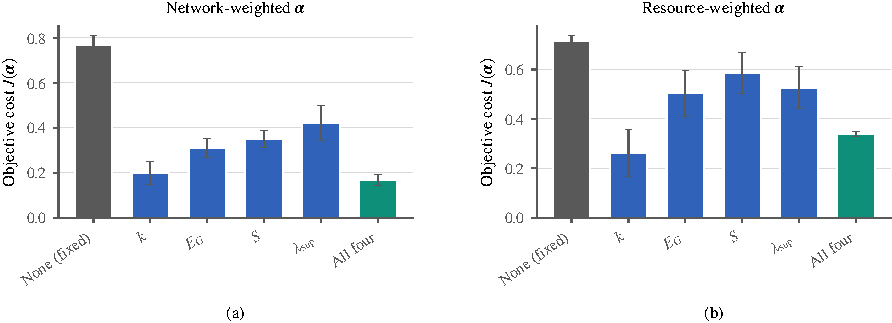
\includegraphics[width=\textwidth]{fig10_knobs.pdf}
\caption{Controller ablation under (a) the network-oriented and (b) the
resource-constrained weighting: objective cost with one variable enabled at a
time (95\% confidence intervals over five seeds).}
\label{fig:knobs}
\end{figure*}

\subsection{Component Ablation}
\label{sec:ablation}
Table~\ref{tab:ablation} and Fig.~\ref{fig:ablation} give the leave-one-out
analysis of the training framework at the fixed configuration. Only one
component produces a large and unambiguous effect: removing context
conditioning -- training an unconditional $G(z)$ -- degrades RMSE by $0.225$
and CRPS by $0.31$, collapses mode coverage to $0.13$, and the model never
reaches the accuracy target. Seed standard deviation is $\approx0.030$ RMSE,
and every coordination component lies within one standard deviation of the full
framework: none of RL-based selection, ensemble feedback or online epoch
adaptation is individually distinguishable at $n=5$. The coordination
mechanisms matter chiefly through cost rather than terminal accuracy: removing
the game-theoretic coordinator raises compute-to-target from $208$ to $334$ work
units and RMSE by $0.027$, but \emph{improves} CRPS, because the fixed schedule
it replaces uses fewer generator epochs. Removing the supervised term raises
compute-to-target to $519$ units ($16.4$ rounds against $7.0$), while
calibration improves (PICP $0.68$); removing the adversarial term gives the
best RMSE of any arm ($0.764$) and the worst calibration ($0.17$) -- a plain
regressor beats the GAN on the metric that rewards collapsing to the mean,
which is why RMSE is not the headline metric here. After Holm correction no
coordination component differs significantly from the full framework on any
accuracy metric.

\begin{table*}[!t]
\centering
\caption{Component ablation at the fixed configuration. Mean\,$\pm$\,s.d.\ over
five seeds; compute is work to first reach RMSE $\le0.86$. No coordination
component differs significantly from the full framework after Holm correction;
only context conditioning does.}
\label{tab:ablation}
\begin{tabular}{lcccccc}
\toprule
Variant & RMSE $\downarrow$ & CRPS $\downarrow$ & minADE $\downarrow$ & PICP $\rightarrow0.90$ & Coverage $\uparrow$ & Compute $\downarrow$ \\
\midrule
\textbf{Full framework (DQN, mean supervision)} & 0.775\,$\pm$\,0.030 & 0.408\,$\pm$\,0.021 & 1.194\,$\pm$\,0.059 & 0.222\,$\pm$\,0.028 & 0.912 & 208 \\
w/o RL-based selection (random-$k$) & 0.778\,$\pm$\,0.032 & 0.410\,$\pm$\,0.018 & 1.199\,$\pm$\,0.049 & 0.220\,$\pm$\,0.013 & 0.907 & 196 \\
w/o ensemble feedback (single critic) & 0.780\,$\pm$\,0.026 & 0.413\,$\pm$\,0.015 & 1.200\,$\pm$\,0.038 & 0.227\,$\pm$\,0.014 & 0.921 & 253 \\
w/o online epoch adaptation (static game) & 0.776\,$\pm$\,0.030 & 0.395\,$\pm$\,0.021 & 1.158\,$\pm$\,0.054 & 0.238\,$\pm$\,0.034 & 0.916 & 210 \\
w/o game coordination (fixed $E_D,E_G$) & 0.802\,$\pm$\,0.033 & 0.384\,$\pm$\,0.020 & 1.149\,$\pm$\,0.056 & 0.336\,$\pm$\,0.037 & 0.954 & 334 \\
Performance-weighted ensemble & 0.775\,$\pm$\,0.030 & 0.408\,$\pm$\,0.023 & 1.193\,$\pm$\,0.061 & 0.220\,$\pm$\,0.029 & 0.912 & 208 \\
w/o supervised term & 0.795\,$\pm$\,0.032 & 0.393\,$\pm$\,0.023 & 1.085\,$\pm$\,0.052 & 0.684\,$\pm$\,0.020 & 0.924 & 519 \\
w/o adversarial term (supervised only) & 0.764\,$\pm$\,0.029 & 0.413\,$\pm$\,0.018 & 1.192\,$\pm$\,0.051 & 0.166\,$\pm$\,0.016 & 0.884 & 155 \\
All coordination removed & 0.820\,$\pm$\,0.031 & 0.390\,$\pm$\,0.019 & 1.175\,$\pm$\,0.051 & 0.352\,$\pm$\,0.047 & 0.950 & 184 \\
\midrule
w/o context conditioning ($G(z)$) & 1.000\,$\pm$\,0.022 & 0.720\,$\pm$\,0.021 & 1.949\,$\pm$\,0.045 & 0.137\,$\pm$\,0.024 & 0.131 & never \\
\bottomrule
\end{tabular}
\end{table*}

\begin{figure*}[!t]
\centering
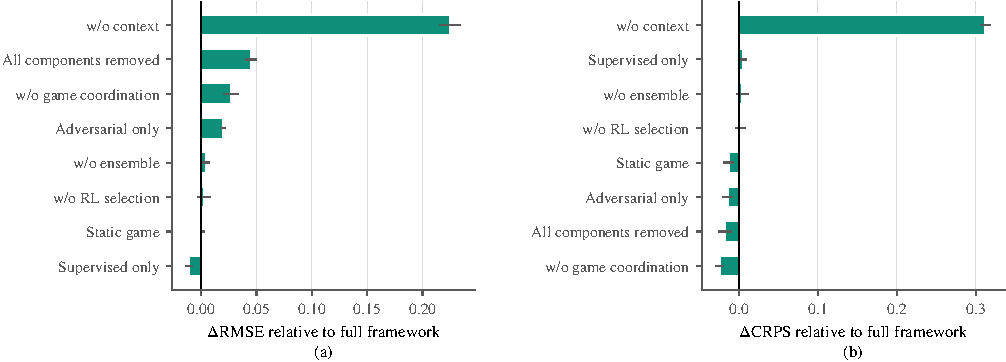
\includegraphics[width=\textwidth]{fig3_ablation.pdf}
\caption{Component ablation: change in (a) RMSE and (b) CRPS when each
component is removed, relative to the full framework. Positive values indicate
that removal degrades performance; error bars are 95\% confidence intervals
over five seeds. Only context conditioning is unambiguously large on both
metrics.}
\label{fig:ablation}
\end{figure*}

\subsection{Discriminator Selection Strategies}
\label{sec:selection}
Table~\ref{tab:selection} compares eight selection strategies with everything
else held fixed. In the main configuration (pool of five per RSU, $k=3$) no
pair differs significantly on any accuracy metric: the learned DQN policy, a
genetic and a lazy-greedy set search, a residence-aware rule and three trivial
rules all lie within $0.006$ RMSE and $0.010$ CRPS of one another. Activating
the whole pool reaches the target in slightly fewer rounds at $31\%$ more
compute and $69\%$ more traffic. Reward weightings $(w_1,\ldots,w_5)$ emphasising
accuracy, delay, resources or traffic in~(\ref{eq:reward}) produce identical
results to the balanced weighting, which is consistent: when selection does not
change the outcome, the reward that drives it cannot either.

A supplementary configuration with a larger pool (ten vehicles per RSU,
$k=3$, 40 rounds, six seeds) gives a different picture: there the DQN beats
greedy-by-loss on all four accuracy metrics (RMSE $0.853$ versus $0.863$,
CRPS $0.403$ versus $0.421$, minADE $1.097$ versus $1.136$, PICP $0.717$
versus $0.687$; paired $p=0.031$, the smallest value attainable at $n=6$) and
is the only strategy to improve calibration significantly, while the set-search
strategies fall between the two. The honest statement is therefore conditional:
learned selection pays off in proportion to the size and heterogeneity of the
candidate pool, and in the bounded pools of the main study it does not. This is
also the reason the controller of Section~\ref{sec:controller} is a closed-form
map rather than another learned policy.

\begin{table}[!t]
\centering
\caption{Discriminator-selection strategies under an otherwise identical
framework (pool of five, $k=3$). Mean\,$\pm$\,s.d.\ over five seeds; rounds and
compute are the cost of reaching RMSE $\le0.86$.}
\label{tab:selection}
\footnotesize
\begin{tabular}{lcccrr}
\toprule
Strategy & RMSE $\downarrow$ & CRPS $\downarrow$ & PICP & Rounds & Compute \\
\midrule
DQN (deep RL) & 0.775\,$\pm$\,0.030 & 0.408\,$\pm$\,0.021 & 0.222 & 7.0 & 208 \\
Greedy-by-loss & 0.774\,$\pm$\,0.030 & 0.417\,$\pm$\,0.022 & 0.235 & 6.4 & 188 \\
Lazy-greedy (set) & 0.778\,$\pm$\,0.033 & 0.410\,$\pm$\,0.022 & 0.214 & 6.6 & 199 \\
Genetic (set) & 0.779\,$\pm$\,0.029 & 0.412\,$\pm$\,0.017 & 0.221 & 6.6 & 197 \\
Residence-aware & 0.779\,$\pm$\,0.030 & 0.412\,$\pm$\,0.017 & 0.219 & 6.6 & 196 \\
Round-robin & 0.774\,$\pm$\,0.030 & 0.407\,$\pm$\,0.019 & 0.230 & 6.4 & 188 \\
Random-$k$ & 0.778\,$\pm$\,0.032 & 0.410\,$\pm$\,0.018 & 0.220 & 6.6 & 196 \\
All discriminators & 0.773\,$\pm$\,0.030 & 0.414\,$\pm$\,0.018 & 0.231 & 5.2 & 247 \\
\bottomrule
\end{tabular}
\end{table}

\subsection{Calibration and Predictive Diversity}
\label{sec:calibration}
Table~\ref{tab:diversity} and Fig.~\ref{fig:calib} isolate the supervision
mechanism of~(\ref{eq:sup}). With conditional-mean supervision the generator
ignores its latent input: its nominal $90\%$ interval covers $22\%$ of targets.
Mode-seeking regularisation~\cite{mao2019msgan} raises PICP to $0.61$ at
$\lambda_{\rm div}=1$ and attains the best CRPS ($0.384$); best-of-$k_s$
supervision raises PICP to $0.70$--$0.77$ and attains the best minADE
($1.052$ at $k_s=4$), at unchanged RMSE. The released configuration uses
best-of-$k_s$ with $k_s=8$, trading a CRPS difference inside seed variance for
a substantially better-calibrated interval. This is the single most important
repair in the training model, and it is invisible to RMSE and MAE.

\begin{table}[!t]
\centering
\caption{Effect of the diversity mechanism on calibration (five seeds). MS:
mode-seeking regulariser with weight $\lambda_{\rm div}$; BoK: best-of-$k_s$
supervision.}
\label{tab:diversity}
\footnotesize
\begin{tabular}{lcccc}
\toprule
Mechanism & PICP $\rightarrow0.90$ & CRPS $\downarrow$ & minADE $\downarrow$ & RMSE $\downarrow$ \\
\midrule
None (conditional-mean) & 0.222\,$\pm$\,0.028 & 0.408\,$\pm$\,0.021 & 1.194\,$\pm$\,0.059 & 0.775 \\
MS, $\lambda_{\rm div}=0.1$ & 0.275\,$\pm$\,0.028 & 0.406\,$\pm$\,0.018 & 1.188\,$\pm$\,0.049 & 0.776 \\
MS, $\lambda_{\rm div}=0.5$ & 0.482\,$\pm$\,0.026 & 0.391\,$\pm$\,0.019 & 1.133\,$\pm$\,0.052 & 0.774 \\
MS, $\lambda_{\rm div}=1.0$ & 0.610\,$\pm$\,0.021 & \textbf{0.384\,$\pm$\,0.020} & 1.100\,$\pm$\,0.048 & 0.774 \\
BoK, $k_s=4$ & 0.699\,$\pm$\,0.016 & 0.385\,$\pm$\,0.019 & \textbf{1.052\,$\pm$\,0.045} & 0.776 \\
BoK, $k_s=8$ & 0.734\,$\pm$\,0.023 & 0.394\,$\pm$\,0.020 & 1.065\,$\pm$\,0.045 & 0.779 \\
BoK, $k_s=16$ & \textbf{0.765\,$\pm$\,0.012} & 0.400\,$\pm$\,0.020 & 1.089\,$\pm$\,0.042 & 0.780 \\
BoK $k_s=8$ + MS 0.5 & 0.776\,$\pm$\,0.010 & 0.399\,$\pm$\,0.019 & 1.081\,$\pm$\,0.037 & 0.778 \\
\bottomrule
\end{tabular}
\end{table}

\begin{figure*}[!t]
\centering
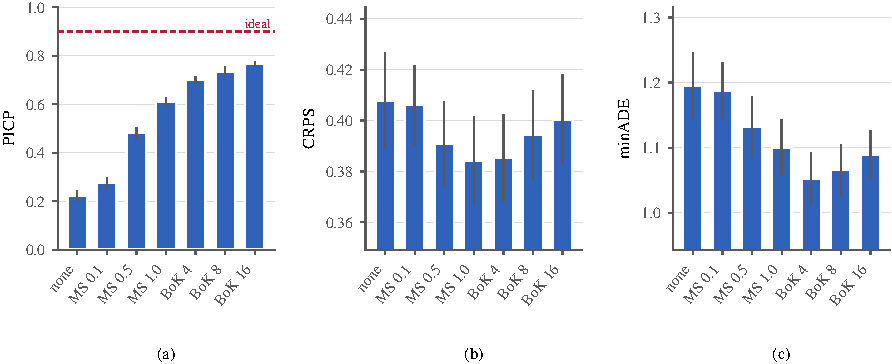
\includegraphics[width=\textwidth]{fig4_calibration.pdf}
\caption{Effect of the diversity mechanism on (a) interval calibration,
(b) CRPS and (c) minADE. Panels (b) and (c) use a non-zero baseline; the plotted
range is a few percent of the value.}
\label{fig:calib}
\end{figure*}

\subsection{Sensitivity Analysis}
\label{sec:sensitivity}
Fig.~\ref{fig:sens} sweeps the active subset size $k$, the supervision weight
$\lambda_{\rm sup}$ and the interference coefficient $\gamma$ of the
coordination game; Table~\ref{tab:scale} gives the resource side of the $k$
sweep. CRPS is smooth in $k$ with a shallow minimum at $k=2$--$3$, while
traffic grows from $4.6$ to $28.4$\,MB per round, latency from $0.97$ to
$3.39$\,s and compute-to-target from $129$ to $279$ units as $k$ goes from one
to five: this monotone, opposite-signed behaviour is the direction entry for
$k$ in Table~\ref{tab:ctrl}, and it is why $k$ is the most effective variable
in Section~\ref{sec:knobs}. The supervision weight governs the
accuracy/calibration trade-off directly: RMSE improves from $0.795$ to $0.767$
as $\lambda_{\rm sup}$ goes from $0$ to $25$ while PICP falls from $0.69$ to
$0.20$, and CRPS is best at $\lambda_{\rm sup}=1$. \textbf{The interference
coefficient has no measurable effect} on any metric across its full range; we
report this null result about a parameter the formulation introduces rather than
omit it. A preliminary generator-budget sweep behind the $E_G$ direction shows an
interior optimum in cost-to-target ($E_G=15$: $707$ units; $E_G=5$: $810$; $E_G=25$:
$768$) with CRPS best at the smallest budget, the trade-off the controller
exploits.

\begin{figure*}[!t]
\centering
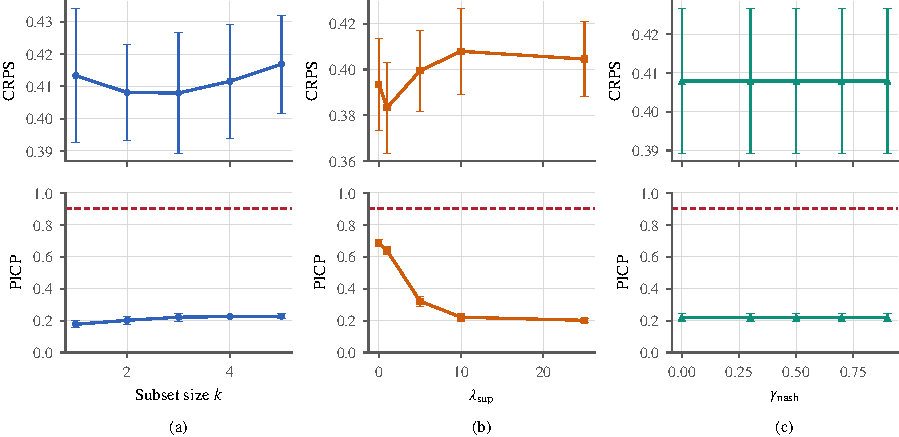
\includegraphics[width=\textwidth]{fig6_sensitivity.pdf}
\caption{Sensitivity of CRPS (top) and PICP (bottom) to (a) the active subset
size $k$, (b) the supervision weight $\lambda_{\rm sup}$ and (c) the
interference coefficient $\gamma$, which has no measurable effect. Error bars
are 95\% confidence intervals over five seeds.}
\label{fig:sens}
\end{figure*}

\subsection{Data Partitioning}
\label{sec:partition}
Table~\ref{tab:partition} evaluates the partitioning of trajectories across
discriminators. Road-segment partitioning, used throughout, gives the best
point and multi-modal accuracy and the fastest convergence; lane partitioning is
comparable in accuracy but converges more slowly; natural
per-track and shuffled partitions, which are statistically near-identical
across nodes, converge three times more slowly and one seed in five never
reaches the target. The partitioning determines whether there is anything for
a selection or adaptation mechanism to exploit, which is why it is reported.

\begin{table}[!t]
\centering
\caption{Effect of the data partitioning across discriminators. Rounds and
compute are the cost of first reaching RMSE $\le0.86$, with the fraction of
seeds reaching it.}
\label{tab:partition}
\footnotesize
\begin{tabular}{lcccc}
\toprule
Partitioning & RMSE $\downarrow$ & CRPS $\downarrow$ & Rounds $\downarrow$ & Compute $\downarrow$ \\
\midrule
Road segment (used) & 0.775\,$\pm$\,0.030 & 0.408\,$\pm$\,0.021 & 7.0 & 208 \\
Lane & 0.794\,$\pm$\,0.015 & 0.416\,$\pm$\,0.016 & 11.4 & 174 \\
Natural (per-track) & 0.832\,$\pm$\,0.030 & 0.396\,$\pm$\,0.009 & 20.8 (4/5) & 655 \\
Shuffled & 0.832\,$\pm$\,0.030 & 0.397\,$\pm$\,0.009 & 20.2 (4/5) & 638 \\
IID split & 0.806\,$\pm$\,0.025 & 0.429\,$\pm$\,0.018 & 14.4 & 444 \\
\bottomrule
\end{tabular}
\end{table}

\subsection{Scalability}
\label{sec:scalability}
\subsubsection{Deployment Scale}
Table~\ref{tab:scale} scales the RSU count, the local pool and the active
subset. Per-round traffic is invariant to $N_G$ and pool size and linear in
$k$, as the $\mathcal{O}(S_{\rm sync}N_GK_Sd)$ analysis predicts for one RSU.
Accuracy degrades with more RSUs sharing the single NGSIM site -- each
road-segment shard holds fewer tracks as the site is cut more finely -- and
compute-to-target rises accordingly. The sweep is bounded at 30 vehicles for
that reason, which we state rather than extrapolate beyond.

\begin{table}[!t]
\centering
\caption{Scaling the deployment: RSU count $N_G$, local pool size, and active
subset $k$ (all else as in Table~\ref{tab:sim}). Traffic is the mean per-round
exchange per RSU; compute is work to first reach RMSE $\le0.86$ with the
fraction of seeds reaching it.}
\label{tab:scale}
\footnotesize
\begin{tabular}{lcccc}
\toprule
Setting & RMSE $\downarrow$ & CRPS $\downarrow$ & Compute $\downarrow$ & Traffic (MB) \\
\midrule
$N_G=2$ (10 vehicles) & 0.775\,$\pm$\,0.030 & 0.408\,$\pm$\,0.021 & 208 & 16.8 \\
$N_G=4$ (20 vehicles) & 0.857\,$\pm$\,0.093 & 0.449\,$\pm$\,0.040 & 1041 (4/5) & 16.8 \\
$N_G=6$ (30 vehicles) & 0.804\,$\pm$\,0.032 & 0.441\,$\pm$\,0.017 & 938 & 16.8 \\
\midrule
Pool 3 per RSU & 0.869\,$\pm$\,0.095 & 0.434\,$\pm$\,0.029 & 226 (2/5) & 16.9 \\
Pool 5 per RSU & 0.775\,$\pm$\,0.030 & 0.408\,$\pm$\,0.021 & 208 & 16.8 \\
Pool 8 per RSU & 0.823\,$\pm$\,0.071 & 0.423\,$\pm$\,0.029 & 574 (4/5) & 16.7 \\
\midrule
$k=1$ & 0.782\,$\pm$\,0.032 & 0.413\,$\pm$\,0.024 & 129 & 4.6 \\
$k=2$ & 0.776\,$\pm$\,0.024 & 0.408\,$\pm$\,0.017 & 176 & 10.8 \\
$k=3$ & 0.775\,$\pm$\,0.030 & 0.408\,$\pm$\,0.021 & 208 & 16.8 \\
$k=4$ & 0.775\,$\pm$\,0.031 & 0.412\,$\pm$\,0.020 & 259 & 22.7 \\
$k=5$ & 0.773\,$\pm$\,0.030 & 0.417\,$\pm$\,0.017 & 279 & 28.4 \\
\bottomrule
\end{tabular}
\end{table}

\subsubsection{Accuracy--Cost Trade-off}
Fig.~\ref{fig:pareto} places every evaluated configuration on the CRPS versus
compute-to-target plane. The proposed fixed configuration sits at the low-cost
end of the Pareto frontier; MD-GAN attains the lowest CRPS at $6.8\times$ the
computation. The adaptive configurations of Table~\ref{tab:terms} move along
this frontier according to $\valpha$ rather than occupying one point of it.

\begin{figure}[!t]
\centering
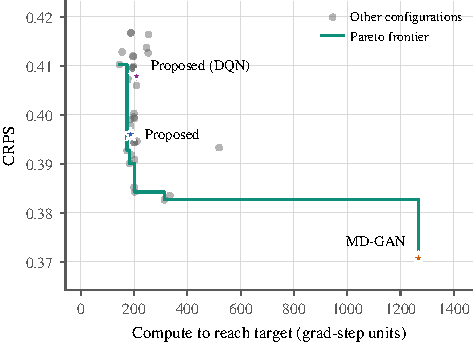
\includegraphics[width=\columnwidth]{fig5_pareto.pdf}
\caption{Accuracy versus cost across all evaluated configurations, with the
Pareto frontier. The proposed fixed configuration sits at the low-cost end;
MD-GAN attains lower CRPS at substantially higher computation.}
\label{fig:pareto}
\end{figure}

\subsubsection{Communication Measurements over IEEE 802.11p}
\label{sec:comm}
Fig.~\ref{fig:ns3} reports the synchronisation round measured in ns-3 over the
IEEE 802.11p stack of Table~\ref{tab:sim}: RSUs broadcast a payload to their
$k$ selected vehicles and wait for the replies. Round latency grows from
$15$ to $25$\,ms as the vehicle population grows from 8 to 40, from $8$ to
$40$\,ms as the selected subset grows from one to five, and from $12$ to
$34$\,ms as the RSU count grows from two to eight -- approximately linear in
$k$ and $N_G$, consistent with the analysis of Section~\ref{sec:complexity},
and the two factors the controller acts on. Delivery ratio is reported alongside
latency because the two cannot be read separately: $35$--$52\%$ of expected
replies arrive within the round at $600$\,m, falling to $32\%$ at eight RSUs
as contention between simultaneous broadcasts increases. At the $1500$\,m
mobility area of our earlier setup, delivery falls to $1$--$8\%$ because most
vehicles are outside 802.11p range of any RSU, and the apparent latency of
$3$--$6$\,ms describes only the few near-range links that complete; reporting
latency without delivery ratio would be misleading, and the $600$\,m deployment
is the regime the framework targets. These packet-level latencies are tens of
milliseconds; the $1$--$2$\,s round latencies of Table~\ref{tab:metrics}
additionally include the compute time of the round and are the quantity the
objective weights.

\begin{figure*}[!t]
\centering
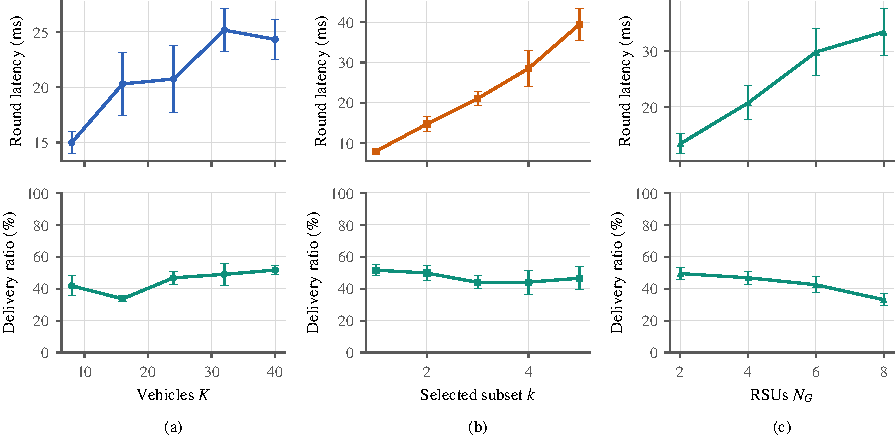
\includegraphics[width=\textwidth]{fig7_ns3_scalability.pdf}
\caption{Measured IEEE 802.11p behaviour of one synchronisation round in ns-3:
round latency (top) and delivery ratio (bottom) versus (a) vehicle count,
(b) selected subset size and (c) RSU count, for a 600\,m deployment (95\%
confidence intervals over five seeds).}
\label{fig:ns3}
\end{figure*}

% =====================================================================
\section{Discussion and Limitations}
\label{sec:discussion}
Several qualifications bound the results above, and we state them explicitly.

\emph{Statistical resolution.} With five seeds the smallest attainable paired
$p$ is $0.062$; every adaptive-versus-fixed comparison attains it with a
consistent direction across all seeds, but none clears the conventional
$0.05$. The effect sizes -- $35$--$85\%$ of the cost -- are large relative to
seed variance, and the released harness is resumable, so the comparison can be
extended to more seeds without re-running the sweep.

\emph{Direction model.} The cost directions of Table~\ref{tab:ctrl} are
measured signs and relative magnitudes, not learned, and they are linear: the
controller ablation shows that this misrepresents the interaction between
variables under the resource weighting. A quadratic or data-driven direction
model would likely close that gap.

\emph{Baselines at fixed configurations.} The baselines are run at their
published configurations. The variables the controller moves exist in any
federated GAN, and equipping a baseline with an equivalent controller is the
natural follow-up; the present comparison establishes that a deployment stating
its objective is served better by using it than by any fixed configuration,
including our own.

\emph{What adaptation costs.} The adaptive configurations hold CRPS at the
level of the best baseline but give up point error (RMSE $0.84$ versus $0.78$)
and some calibration relative to our fixed configuration. The objective weights
decide whether that trade is acceptable; the accuracy-oriented column shows the
controller spending more when it is not.

\emph{Metrics.} Compute counts gradient steps, so a configuration that trains
less scores better on three of the five terms; only the training term pushes
back. Round latency in the training-time model includes compute time and is
not comparable with the packet-level ns-3 figures. The $0.86$ accuracy target
was chosen after inspecting the data; Fig.~\ref{fig:conv} shows the full
curves so the choice can be checked against any threshold.

\emph{Scope.} The evaluation is single-step prediction on one dataset, with
deployment scale bounded by the available NGSIM partitions, and our earlier
early-update MD-GAN was not ported into the common protocol.

% =====================================================================
\section{Conclusion}
\label{sec:conclusion}
This paper presented an objective-adaptive multi-discriminator WGAN framework
for resource-constrained IoV in which the deployment's own weight vector is an
input to the training configuration rather than only a reporting convention.
Four configuration variables that drive distinct terms of a unified objective --
the active critic subset, the generator epoch budget, the synchronisation
interval and the supervision weight -- are set by projecting the weight vector
onto measured cost directions, at negligible cost, with an online dual update
as an explored alternative. Against three federated GAN baselines
re-implemented under one protocol on real NGSIM trajectories, the adaptive
framework attains the lowest objective cost under all five deployment
weightings evaluated, improving on the strongest baseline by $35$--$75\%$ and
on our own fixed configuration by $58$--$85\%$, while holding distributional
accuracy at the level of the best baseline and cutting per-round traffic by an
order of magnitude. The conditional training model reaches a target accuracy
$5.6\times$ faster than MD-GAN at $6.8\times$ less computation and yields a far
better-calibrated predictive distribution.

The study also establishes what does \emph{not} determine outcomes in this
setting: no participant-selection strategy among eight, learned or heuristic,
is distinguishable at bounded pool sizes; no coordination component is
individually distinguishable from the full framework at five seeds; the
interference coefficient of the coordination game has no measurable effect;
and merely knowing the objective is worth more than tracking it online in four
of five weightings. Predictive quality is dominated by conditioning the
generator on trajectory context and by the design of the supervision term.
Future work will model interaction between configuration variables, extend the
evaluation to multi-step prediction and larger partitions, and equip the
baselines with equivalent controllers so that the benefit of objective
adaptation can be separated from the architecture that hosts it.

% =====================================================================
\begin{thebibliography}{99}

\bibitem{pratap2023cotev}
S.~Pratap, P.~Dass, and S.~Misra, ``CoTEV: Trustworthy and cooperative task
execution in Internet of Vehicles,'' \emph{IEEE Trans. Mobile Comput.},
vol.~23, no.~4, pp.~2915--2926, 2023.

\bibitem{devika2024vadgan}
S.~Devika, R.~R. Shrivastava, P.~Narang, T.~Alladi, and F.~R. Yu, ``VADGAN: An
unsupervised GAN framework for enhanced anomaly detection in connected and
autonomous vehicles,'' \emph{IEEE Trans. Veh. Technol.}, vol.~73, no.~9,
pp.~12\,458--12\,467, 2024.

\bibitem{zhang2023fedgan}
J.~Zhang, L.~Zhao, K.~Yu, G.~Min, A.~Y. Al-Dubai, and A.~Y. Zomaya, ``A novel
federated learning scheme for generative adversarial networks,'' \emph{IEEE
Trans. Mobile Comput.}, vol.~23, no.~5, pp.~3633--3649, 2023.

\bibitem{mishra2023dew}
K.~Mishra, G.~N. Rajareddy, U.~Ghugar, G.~S. Chhabra, and A.~H. Gandomi, ``A
collaborative computation and offloading for compute-intensive and
latency-sensitive dependency-aware tasks in dew-enabled vehicular fog
computing: A federated deep Q-learning approach,'' \emph{IEEE Trans. Netw.
Service Manag.}, vol.~20, no.~4, pp.~4600--4614, 2023.

\bibitem{kaleibar2026semantic}
F.~J. Kaleibar, M.~St-Hilaire, and M.~Barati, ``A novel architectural framework
for semantic-based service provisioning in vehicular cloud networks,''
\emph{IEEE Trans. Services Comput.}, pp.~1--14, 2026.

\bibitem{mfogo2025ganaiipot}
V.~S. Mfogo, A.~Zemkoho, L.~Njilla, M.~J. Nkenlifack, and C.~A. Kamhoua,
``GAN-AIIPot: GAN-based cyber deception for probing attacks on IoT devices,''
\emph{IEEE Trans. Netw. Service Manag.}, vol.~23, pp.~417--431, 2025.

\bibitem{luo2025wgan}
X.~Luo, Z.~Wei, G.~Zhang, H.~Huang, and R.~Zhou, ``High-risk powered
two-wheelers scenarios generation for autonomous vehicle testing using WGAN,''
\emph{Traffic Injury Prevention}, vol.~26, no.~2, pp.~243--251, 2025.

\bibitem{zaki2026mambavec}
A.~M. Zaki, S.~A. Elsayed, K.~Elgazzar, H.~S. Hassanein, and S.~Moussa,
``MambaVEC: A multi-agent DRL framework with Mamba for efficient long-term
vehicular edge computing task offloading,'' in \emph{Proc. Int. Conf. Smart
Mobility (SM)}, 2026, pp.~1--7.

\bibitem{contreras2025genai}
J.~Contreras-Castillo, J.~Guerrero-Iba\~{n}ez, S.~Zeadally, and E.-K. Hong,
``Generative AI for Internet of Vehicles (IoV): Potential and challenges,''
\emph{IEEE Commun. Standards Mag.}, 2025.

\bibitem{kaleibar2024clustering}
F.~J. Kaleibar and M.~St-Hilaire, ``An adaptive clustering approach for dynamic
service provisioning in vehicular cloud networks,'' in \emph{Proc. IEEE World
Forum Internet of Things (WF-IoT)}, 2024, pp.~666--671.

\bibitem{hammoud2022fog}
A.~Hammoud, M.~Kantardjian, A.~Najjar, A.~Mourad, H.~Otrok, Z.~Dziong, and
N.~Guizani, ``Dynamic fog federation scheme for Internet of Vehicles,''
\emph{IEEE Trans. Netw. Service Manag.}, vol.~20, no.~2, pp.~1913--1923, 2022.

\bibitem{yuan2020controller}
T.~Yuan, W.~da Rocha Neto, C.~E. Rothenberg, K.~Obraczka, C.~Barakat, and
T.~Turletti, ``Dynamic controller assignment in software defined Internet of
Vehicles through multi-agent deep reinforcement learning,'' \emph{IEEE Trans.
Netw. Service Manag.}, vol.~18, no.~1, pp.~585--596, 2020.

\bibitem{karim2022architecture}
S.~M. Karim, A.~Habbal, S.~A. Chaudhry, and A.~Irshad, ``Architecture,
protocols, and security in IoV: Taxonomy, analysis, challenges, and
solutions,'' \emph{Security and Communication Networks}, vol.~2022, no.~1,
p.~1131479, 2022.

\bibitem{elbir2022fl}
A.~M. Elbir, B.~Soner, S.~\c{C}oleri, D.~G\"{u}nd\"{u}z, and M.~Bennis,
``Federated learning in vehicular networks,'' in \emph{Proc. IEEE
MeditCom}, 2022, pp.~72--77.

\bibitem{wang2022joint}
G.~Wang, F.~Xu, H.~Zhang, and C.~Zhao, ``Joint resource management for mobility
supported federated learning in Internet of Vehicles,'' \emph{Future Gener.
Comput. Syst.}, vol.~129, pp.~199--211, 2022.

\bibitem{posner2021fl}
J.~Posner, L.~Tseng, M.~Aloqaily, and Y.~Jararweh, ``Federated learning in
vehicular networks: Opportunities and solutions,'' \emph{IEEE Netw.}, vol.~35,
no.~2, pp.~152--159, 2021.

\bibitem{kaleibar2025genetic}
F.~J. Kaleibar, M.~St-Hilaire, and M.~Barati, ``A customized genetic algorithm
for SLA-aware service provisioning in infrastructure-less vehicular cloud
networks,'' \emph{IEEE Trans. Services Comput.}, vol.~18, pp.~499--512, 2025.

\bibitem{wang2022mdbiwgan}
W.~Wang, C.~Liang, L.~Tang, H.~Yanikomeroglu, and Q.~Chen, ``Federated
multi-discriminator BiWGAN-GP based collaborative anomaly detection for
virtualized network slicing,'' \emph{IEEE Trans. Mobile Comput.}, vol.~22,
no.~11, pp.~6445--6459, 2022.

\bibitem{wu2024hvsgan}
L.~Wu, H.~Lin, and X.~Wang, ``Federated training generative adversarial
networks for heterogeneous vehicle scheduling in IoV,'' \emph{IEEE Internet
Things J.}, 2024.

\bibitem{xie2024gaiiov}
G.~Xie, Z.~Xiong, X.~Zhang, R.~Xie, S.~Guo, M.~Guizani, and H.~V. Poor,
``GAI-IoV: Bridging generative AI and vehicular networks for ubiquitous edge
intelligence,'' \emph{IEEE Trans. Wireless Commun.}, vol.~23, no.~10,
pp.~12\,799--12\,814, 2024.

\bibitem{quan2024fl}
H.~Quan, Q.~Zhang, and J.~Zhao, ``Federated learning assisted intelligent IoV
mobile edge computing,'' \emph{IEEE Trans. Green Commun. Netw.}, vol.~9, no.~1,
pp.~228--241, 2024.

\bibitem{hazarika2023ris}
B.~Hazarika, K.~Singh, S.~Biswas, S.~Mumtaz, and C.-P. Li, ``Multi-agent
DRL-based task offloading in multiple RIS-aided IoV networks,'' \emph{IEEE
Trans. Veh. Technol.}, vol.~73, no.~1, pp.~1175--1190, 2023.

\bibitem{xu2024caching}
X.~Xu, L.~Gu, M.~Bilal, M.~Khan, Y.~Wen, G.~Liu, and Y.~Yuan, ``Multi-agent
reinforcement learning based edge content caching for connected autonomous
vehicles in IoV,'' \emph{ACM Trans. Auton. Adapt. Syst.}, 2024.

\bibitem{kaleibar2025mascots}
F.~Jafari Kaleibar and M.~Litoiu, ``A distributed GAN-based framework for
low-latency and efficient learning in the Internet of Vehicles,'' in
\emph{Proc. IEEE MASCOTS}, 2025, pp.~1--8.

\bibitem{liang2020rl}
H.~Liang, X.~Zhang, X.~Hong, Z.~Zhang, M.~Li, G.~Hu, and F.~Hou,
``Reinforcement learning enabled dynamic resource allocation in the Internet
of Vehicles,'' \emph{IEEE Trans. Ind. Informat.}, vol.~17, no.~7,
pp.~4957--4967, 2020.

\bibitem{zaki2025cogroup}
A.~M. Zaki, S.~A. Elsayed, K.~Elgazzar, and H.~S. Hassanein, ``CoGroup:
Cooperative quality offloading with worker grouping using hierarchical
multi-agent deep reinforcement learning,'' in \emph{Proc. IWCMC}, 2025,
pp.~1276--1281.

\bibitem{arjovsky2017wgan}
M.~Arjovsky, S.~Chintala, and L.~Bottou, ``Wasserstein GAN,''
\emph{arXiv:1701.07875}, 2017.

\bibitem{hua2019gan}
Y.~Hua, R.~Li, Z.~Zhao, X.~Chen, and H.~Zhang, ``GAN-powered deep
distributional reinforcement learning for resource management in network
slicing,'' \emph{IEEE J. Sel. Areas Commun.}, vol.~38, no.~2, pp.~334--349,
2019.

\bibitem{creswell2018gan}
A.~Creswell, T.~White, V.~Dumoulin, K.~Arulkumaran, B.~Sengupta, and A.~A.
Bharath, ``Generative adversarial networks: An overview,'' \emph{IEEE Signal
Process. Mag.}, vol.~35, no.~1, pp.~53--65, 2018.

\bibitem{malektaji2021migration}
S.~Malektaji, A.~Ebrahimzadeh, H.~Elbiaze, R.~H. Glitho, and S.~Kianpisheh,
``Deep reinforcement learning-based content migration for edge content delivery
networks with vehicular nodes,'' \emph{IEEE Trans. Netw. Service Manag.},
vol.~18, no.~3, pp.~3415--3431, 2021.

\bibitem{zhao2020trajectory}
L.~Zhao, Y.~Liu, A.~Y. Al-Dubai, A.~Y. Zomaya, G.~Min, and A.~Hawbani, ``A
novel generation-adversarial-network-based vehicle trajectory prediction method
for intelligent vehicular networks,'' \emph{IEEE Internet Things J.}, vol.~8,
no.~3, pp.~2066--2077, 2020.

\bibitem{seo2018gids}
E.~Seo, H.~M. Song, and H.~K. Kim, ``GIDS: GAN based intrusion detection system
for in-vehicle network,'' in \emph{Proc. Conf. Privacy, Security and Trust
(PST)}, 2018, pp.~1--6.

\bibitem{ioannou2026ganenergy}
I.~Ioannou and V.~Vassiliou, ``Generative adversarial networks for energy-aware
IoT intrusion detection: Comprehensive benchmark analysis of GAN architectures
with accuracy-per-joule evaluation,'' \emph{Sensors}, vol.~26, no.~3, p.~757,
2026.

\bibitem{liao2025diffusiondrive}
B.~Liao, S.~Chen, H.~Yin, B.~Jiang, C.~Wang, S.~Yan, X.~Zhang, X.~Li,
Y.~Zhang, Q.~Zhang \emph{et al.}, ``DiffusionDrive: Truncated diffusion model
for end-to-end autonomous driving,'' in \emph{Proc. IEEE/CVF CVPR}, 2025,
pp.~12\,037--12\,047.

\bibitem{demiguel2022vae}
M.~\'{A}. De~Miguel, J.~M. Armingol, and F.~Garc\'{i}a, ``Vehicles trajectory
prediction using recurrent VAE network,'' \emph{IEEE Access}, vol.~10,
pp.~32\,742--32\,749, 2022.

\bibitem{lyu2026client}
N.~Lyu, J.~Zhang, Z.~Shen, C.~Chen, Z.~Jiang, Q.~Chen, and M.~Guo, ``Enabling
client-autonomous training optimizations for efficient federated learning,''
\emph{IEEE Trans. Parallel Distrib. Syst.}, 2026.

\bibitem{cha2024client}
N.~Cha and L.~Chang, ``Multi-objective distributed client selection in
federated learning-assisted Internet of Vehicles,'' \emph{Sensors}, vol.~24,
no.~13, p.~4180, 2024.

\bibitem{lu2025clustered}
S.~Lu, H.~Yin, P.~Wang, T.~Zhu, C.~Dai, S.~Dai, and B.~Guo, ``Clustered
federated learning with adaptive pruning for 6G edge-intelligent
transportation,'' \emph{IEEE Trans. Intell. Transp. Syst.}, 2025.

\bibitem{nie2025caching}
X.~Nie, C.~Wang, T.~Zhou, Q.~Zhou, X.~Zhu, and J.~Zhang, ``Mobility-aware
cooperative caching in IoVs based on secure asynchronous federated and deep
reinforcement learning,'' \emph{IEEE Internet Things J.}, 2025.

\bibitem{wang2019adaptive}
S.~Wang, T.~Tuor, T.~Salonidis, K.~K. Leung, C.~Makaya, T.~He, and K.~Chan,
``Adaptive federated learning in resource constrained edge computing
systems,'' \emph{IEEE J. Sel. Areas Commun.}, vol.~37, no.~6,
pp.~1205--1221, 2019.

\bibitem{nishio2019fedcs}
T.~Nishio and R.~Yonetani, ``Client selection for federated learning with
heterogeneous resources in mobile edge,'' in \emph{Proc. IEEE ICC}, 2019,
pp.~1--7.

\bibitem{chen2021joint}
M.~Chen, Z.~Yang, W.~Saad, C.~Yin, H.~V. Poor, and S.~Cui, ``A joint learning
and communications framework for federated learning over wireless networks,''
\emph{IEEE Trans. Wireless Commun.}, vol.~20, no.~1, pp.~269--283, 2021.

\bibitem{hardy2019mdgan}
C.~Hardy, E.~Le~Merrer, and B.~Sericola, ``MD-GAN: Multi-discriminator
generative adversarial networks for distributed datasets,'' in \emph{Proc.
IEEE IPDPS}, 2019, pp.~866--877.

\bibitem{gneiting2007crps}
T.~Gneiting and A.~E. Raftery, ``Strictly proper scoring rules, prediction, and
estimation,'' \emph{J. Amer. Statist. Assoc.}, vol.~102, no.~477,
pp.~359--378, 2007.

\bibitem{gupta2018socialgan}
A.~Gupta, J.~Johnson, L.~Fei-Fei, S.~Savarese, and A.~Alahi, ``Social GAN:
Socially acceptable trajectories with generative adversarial networks,'' in
\emph{Proc. IEEE/CVF CVPR}, 2018, pp.~2255--2264.

\bibitem{mao2019msgan}
Q.~Mao, H.-Y. Lee, H.-Y. Tseng, S.~Ma, and M.-H. Yang, ``Mode seeking
generative adversarial networks for diverse image synthesis,'' in \emph{Proc.
IEEE/CVF CVPR}, 2019, pp.~1429--1437.

\bibitem{boyd2004convex}
S.~Boyd and L.~Vandenberghe, \emph{Convex Optimization}. Cambridge, U.K.:
Cambridge Univ. Press, 2004.

\bibitem{rappaport2002wireless}
T.~S. Rappaport, \emph{Wireless Communications: Principles and Practice},
2nd~ed. Upper Saddle River, NJ, USA: Prentice Hall, 2002.

\bibitem{ngsim}
U.S. Department of Transportation, Federal Highway Administration, ``Next
Generation Simulation (NGSIM) vehicle trajectories and supporting data,''
2016. [Online]. Available:
\url{https://data.transportation.gov/stories/s/i5zb-xe34}

\end{thebibliography}

\end{document}
